\section{Formulação dos problemas auxiliares e solução via Transformação Integral Clássica}\label{secao_probs_aux}

Será apresentada agora a formulação matemática dos problemas auxiliares cujas soluções fornecem as classes de funções auxiliares $F_1$ e $G_1$, necessárias
para obtenção da estimativa do perfil de CTC através da equação \eqref{equacao_definicao_f_r}. As soluções desses problemas serão desenvolvidas analiticamente através do
emprego da Técnica da Transformada Integral Clássica (CITT). 

Os problemas auxiliares são definidos com base nos problemas apresentados no artigo de \cite{reciproc_2} e modificados por \cite{tese_abreu}.  

\subsection{Primeiro problema auxiliar}\label{secao_do_primeiro}

Sejam duas famílias de funções harmônicas $F_{1, j}$ e $F_{2, j}$, definidas respectivamente nos domínios $\Omega_1$ e $\Omega_2$.Define-se assim o primeiro
problema auxiliar, relacionado ao salto de temperatura na interface $\Gamma$ através das seguintes equações:

\begin{subequations}
	\begin{alignat}{2}
	& \nabla^2 F_{1,j} = 0 \quad\quad\quad\quad\quad && \text{ em } \Omega_1 \label{funcao_F_harm_T1} \\ \nonumber \\
	& F_{1,j} = \psi_j && \text{ em } \Gamma_0  \label{funcao_F_cc_T1_2} \\ \nonumber \\
	& \frac{\partial F_{1,j}}{\partial \mathbf{n}_1} = 0 && \text{ em }  \Gamma_1 \label{funcao_F_cc_T1_1} \\ \nonumber \\
	& F_{1,j} = F_{2, j} \quad\quad\quad\quad\quad\quad\quad\quad && \text{ em }  \Gamma \label{funcao_F_cc_grad_T1} \\ \nonumber \\
	& \nabla^2 F_{2,j} = 0 && \text{ em }  \Omega_2 \label{funcao_F_harm_T2} \\ \nonumber \\
	& \frac{\partial F_{2,j}}{\partial \mathbf{n}_2} = 0 && \text{ em }  \Gamma_2 \label{funcao_F_cc_T1_3} \\ \nonumber \\
	& F_{2,j} = 0 && \text{ em }  \Gamma_\infty \label{funcao_F_cc_T1_4} \\ \nonumber \\
	& k_2\frac{\partial F_{2, j}}{\partial\mathbf{n}_2} = - k_1\frac{\partial F_{1,j}}{\partial\mathbf{n}_1} = -\beta_j && \text{ em }  \Gamma \label{funcao_F_cc_T1_5}
	\end{alignat}
\end{subequations}

Nas equações acima, para compor a condição de contorno na interface superior $\Gamma_0$, foi introduzida uma família de funções $\psi_j(x), j=1,2,\ldots N_1$, a serem definidas posteriormente. A solução do sistema de equações \eqref{funcao_F_harm_T1} a \eqref{funcao_F_cc_T1_5} será escrita em termos daquelas funções. 

\subsection{Segundo problema auxiliar}\label{secao_do_segundo}
Seja a família de funções harmônicas $G_{1, j}$, definida no domínio $\Omega_1$. Define-se assim o segundo
problema auxiliar, relacionado ao fluxo de calor por unidade de área através da interface, $\Gamma$ através das seguintes equações:
\begin{subequations}
	\begin{alignat}{2}
	& \nabla^2 G_{1,j} = 0 \quad\quad\quad\quad\quad && \text{ em } \Omega_1 \label{funcao_G_harm_T1} \\ \nonumber \\
	& G_{1,j} = \phi_j && \text{ em } \Gamma_0  \label{funcao_G_cc_T1_2} \\ \nonumber \\
	& \frac{\partial G_{1,j}}{\partial \mathbf{n}_1} = 0 && \text{ em }  \Gamma_1 \label{funcao_G_cc_T1_1} \\ \nonumber \\
	& \frac{\partial G_{1,j}}{\partial\mathbf{n}_1} = 0 \quad\quad\quad\quad\quad\quad\quad\quad && \text{ em }  \Gamma \label{funcao_G_cc_grad_T1}
	\end{alignat}
\end{subequations}

Assim como no primeiro problema, a fim de compor a condição de contorno na interface superior $\Gamma_0$, foi introduzida uma família de funções $\phi_j(x), j=1,2,\ldots N_2$, que serão definidas posteriormente. A solução do sistema de equações \eqref{funcao_G_harm_T1} a \eqref{funcao_G_cc_grad_T1} será escrita em termos daquelas funções. 

\subsection{Preparação dos problemas auxiliares para aplicação da Técnica da Transformada Integral Clássica}
Os conjuntos de equações \eqref{funcao_F_harm_T1} a \eqref{funcao_F_cc_T1_5} e \eqref{funcao_G_harm_T1} a \eqref{funcao_G_cc_grad_T1}, numa primeira análise,
não estão restritas a algum sistema de coordenadas em particular. Por outro lado, a seção transversal do corpo de prova tem formato retangular; por isso,
a fim de favorecer o uso da Técnica da Transformada Integral Clássica, a ser descrita na próxima seção,
será feita a formulação do problemas auxiliares em termos de coordenadas cartesianas e a redefinição do domínio físico sobre o qual esses problemas
serão resolvidos.

\subsubsection{A Técnica da Transformada Integral Clássica}

A Técnica da Transformada Integral Clássica (do inglês \textit{Classical Integral Transform Technique} - CITT), historicamente baseada no método de separação de variáveis \citep{livro_boyce},
fornece uma abordagem sistemática e eficiente para solução
de problemas difusivos de valor de contorno em regime permanente ou transiente, que envolvam termos não-homogêneos nas equações diferenciais ou nas condições
de contorno \citep{livro_ozisik}. Esta técnica foi recentemente empregada na solução do problema inverso de transferência de calor para determinação da CTC para
uma interface de contato plana, num arranjo semelhante ao da figura \ref{fig4}, fornecendo bons resultados \citep{tese_padilha}. Considerando que o referido problema é um caso particular
de um arranjo mais geral, representado na figura \ref{fig2}, objeto de estudo desta dissertação, foi natural a opção por esta técnica para determinação da solução do problema inverso correspondente.
\begin{figure}[h!b]
\begin{center}
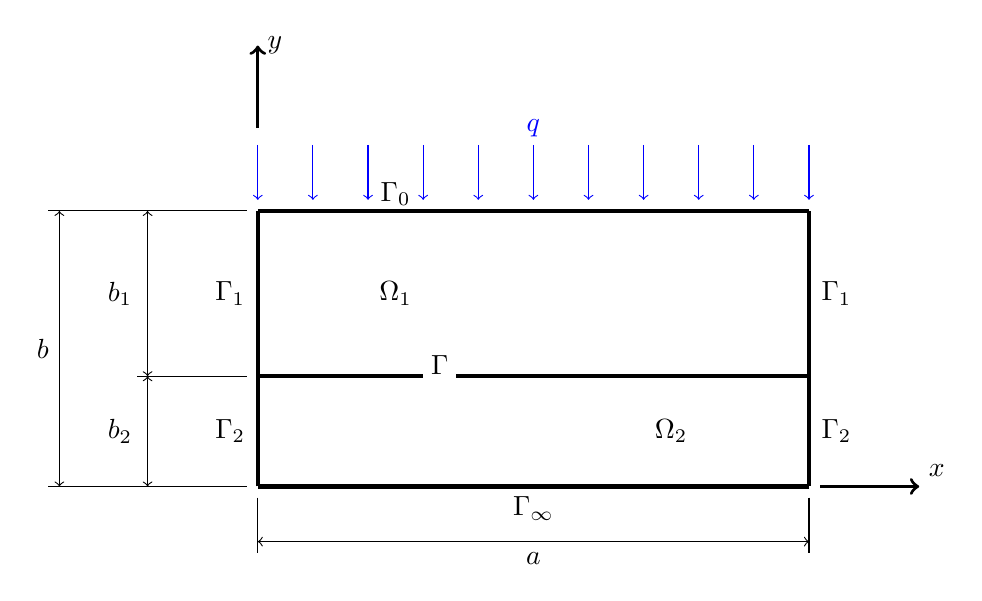
\begin{tikzpicture}[scale=0.7]

	\draw [ultra thick] (0, 0) -- (10, 0);
	%\draw [ultra thick] (0, 2) -- (7, 2);
	%\draw [ultra thick] (8, 2) -- (10, 2);
	\draw [ultra thick] (0, 5) -- (10, 5);
	\draw [ultra thick] (0, 2.0) -- (3.0, 2.0);
	\draw [ultra thick] (3.6, 2.0) -- (10, 2.0);
	\draw [ultra thick] (0, 0) -- (0, 5);
	\draw [ultra thick] (10, 0) -- (10, 5);

	\draw (2.5, 3.5) node {$\Omega_1$};
	\draw (7.5, 1) node {$\Omega_2$};
	\draw (3.3, 2.2) node {$\Gamma$};
	\draw (-0.5, 3.5) node {$\Gamma_1$};
	\draw (-0.5, 1) node {$\Gamma_2$};
	\draw (10.5, 3.5) node {$\Gamma_1$};
	\draw (10.5, 1) node {$\Gamma_2$};
	\draw (5, -0.4) node {$\Gamma_\infty$};
	\draw (2.5, 5.3) node {$\Gamma_0$};
	\draw [blue](5, 6.5) node {$q$};
	\draw (5, -1.3) node {$a$};
	\draw (-3.9, 2.5) node {$b$};
	\draw (-2.5, 1) node {$b_2$};
	\draw (-2.5, 3.5) node {$b_1$};

	\node [above right] at (12, 0) {$x$};
	\node [right] at (0, 8) {$y$};

	\draw [->, blue] (0, 6.2) -- (0, 5.2);
	\draw [->, blue] (1, 6.2) -- (1, 5.2);
	\draw [->, blue] (2, 6.2) -- (2, 5.2);
	\draw [->, blue] (3, 6.2) -- (3, 5.2);
	\draw [->, blue] (4, 6.2) -- (4, 5.2);
	\draw [->, blue] (5, 6.2) -- (5, 5.2);
	\draw [->, blue] (6, 6.2) -- (6, 5.2);
	\draw [->, blue] (7, 6.2) -- (7, 5.2);
	\draw [->, blue] (8, 6.2) -- (8, 5.2);
	\draw [->, blue] (9, 6.2) -- (9, 5.2);
	\draw [->, blue] (10, 6.2) -- (10, 5.2);

	\draw [->, very thick] (10.2,0) -- (12,0);
	\draw [->, very thick] (0, 6.5) -- (0,8);

	\draw [-] (0, -0.2) -- (0, -1.2);
	\draw [-] (10, -0.2) -- (10, -1.2);
	\draw [<->] (0, -1) -- (10, -1);

	\draw [-] (-0.2, 0) -- (-3.8, 0);
	\draw [-] (-0.2, 5) -- (-3.8, 5);
	\draw [-] (-0.2, 2) -- (-2.2, 2);
	\draw [<->] (-3.6, 0) -- (-3.6, 5);
	\draw [<->] (-2.0, 0) -- (-2.0, 2);
	\draw [<->] (-2.0, 2) -- (-2.0, 5);

\end{tikzpicture}
\caption{Geometria do problema físico resolvido por \cite{reciproc_2}}
\label{fig4}
\end{center}
\end{figure}

De acordo com \cite{livro_cotta}, a solução dos problemas via CITT requer a aplicação dos seguintes passos:
\begin{enumerate}[(i)]
	\item Desenvolver o problema de autovalor associado, através da aplicação do método de separação de variáveis à versão homogênea do problema da equação
	diferencial parcial;
	\item Desenvolver o par transformada-inversa apropriado;
	\item Aplicar a transformação integral à equação diferencial parcial do problema de valor de contorno original, empregando as condições de contorno no
	desenvolvimento dos cálculos;
	\item Resolver o sistema de equações diferenciais ordinárias desacopladas gerado a partir da transformação integral; e
	\item Aplicar a fórmula de inversão previamente estabelecida no passo (ii) para construir a solução completa do problema.
\end{enumerate}

Na seção anterior, foi apontada a importância de se definir os problemas auxiliares cuja solução fornece as funções auxiliares $F_{1,j}$ e $G_{1,j}$.
Nas próximas seções, estes problemas serão formulados no sistema de coordenadas cartesianas e resolvidos através da Técnica da Transformada Integral Clássica (CITT). Mas antes, é necessário
expressar em coordenadas cartesianas as derivadas direcionais presentes nas condições de contorno dos problemas auxiliares, o que
será feito a seguir.

\subsubsection{Expressão das derivadas direcionais em coordenadas cartesianas}\label{secao_sobre_normal}
Seja um campo escalar $\Phi$. A derivada direcional em relação ao vetor unitário $\mathbf{u}$ é dada por \citep{livro_stewart_2}:
\begin{align}
& \frac{\partial\Phi}{\partial\mathbf{u}} = \nabla \Phi \cdot \mathbf{u} 
\end{align} 

Em coordenadas cartesianas, havendo dependência apenas de $x$ e $y$, pode-se escrever:
\begin{align}
& \frac{\partial\Phi}{\partial\mathbf{u}} = \frac{\partial \Phi}{\partial x}u_x + \frac{\partial \Phi}{\partial y}u_y\label{derivada_direcional_coodernadas_cartesianas}
\end{align}
onde $u_x$ e $u_y$ são as componentes do vetor unitário $\mathbf{u}$ nas direções $x$ e $y$ respectivamente.

As derivadas direcionais presentes em \eqref{funcao_F_cc_T1_1}, \eqref{funcao_F_cc_T1_3} e \eqref{funcao_G_cc_T1_1}
são em relação a vetores normais unitários paralelos ao eixo $x$ e apontando para fora da superfície que delimita o contorno de $\Omega$. 
Para esses vetores, $u_y = 0$ e $u_x = \pm 1$, dependendo do sentido para onde o vetor aponta. Essas derivadas, pelas condições de contorno, são
todas nulas, por isso o sinal de $u_x$ é indiferente nestes casos. Por exemplo, a condição de contorno \eqref{funcao_F_cc_T1_1} pode
ser escrita como:
\begin{align}
\frac{\partial F_{1,j}(0, y)}{\partial x} = 0, \quad\quad\quad w(0) < y < b 
\end{align}

As equações \eqref{expressao_define_beta}, \eqref{funcao_F_cc_T1_5} e \eqref{funcao_G_cc_grad_T1} possuem derivadas direcionais calculadas sobre a superfície $\Gamma$.
Sejam então os vetores normais $\mathbf{n}_2$ e $\mathbf{n}_1$ em uma dada posição sobre essa superfície, apontando para fora das regiões $\Omega_2$ e $\Omega_1$ respectivamente, e
seja também o vetor tangente $\mathbf{T}$ na mesma posição, em relação à superfície $\Gamma$. Estes vetores estão ilustrados na figura \ref{fig7}.
\begin{figure}[h!b]
	\begin{center}
		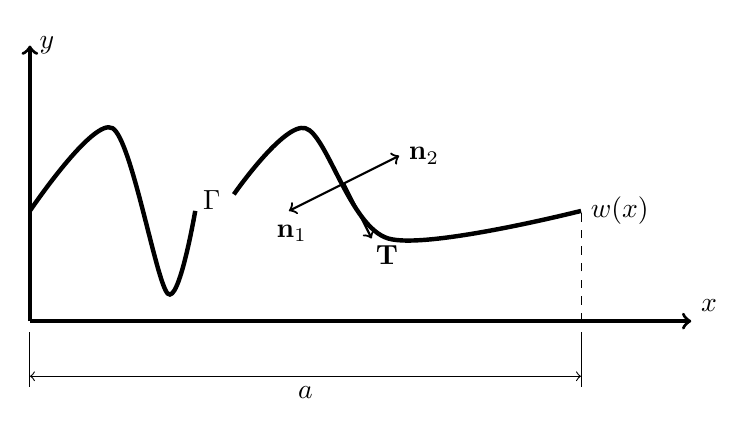
\begin{tikzpicture}[scale=0.7]
		\draw [ultra thick] plot [smooth] coordinates {(0, 2) (1.5, 3.5) (2.5, 0.5) (3, 2)};
		\draw [ultra thick] plot [smooth] coordinates {(3.7, 2.3) (5, 3.5) (6.5, 1.5) (10, 2)};		
		\draw [dashed] (10, 0) -- (10, 2);
		
		\draw (3.3, 2.2) node {$\Gamma$};
		\draw (5, -1.3) node {$a$};
		
		\node [above right] at (12, 0) {$x$};
		\node [right] at (0, 5) {$y$};
		
		\draw [->, thick] (5.7,2.5) -- (4.7,2);
		\node [right] at (4.3, 1.6) {$\mathbf{n}_1$};
		
		\draw [->, thick] (5.7,2.5) -- (6.7,3);
		\node [right] at (6.7, 3) {$\mathbf{n}_2$};
		
		\draw [->, thick] (5.7,2.5) -- (6.2,1.5);
		\node [right] at (6.1, 1.2) {$\mathbf{T}$};
		
		\node [right] at (10, 2) {$w(x)$};
		
		\draw [->, very thick] (0,0) -- (12,0);
		\draw [->, very thick] (0, 0) -- (0,5);
		
		\draw [-] (0, -0.2) -- (0, -1.2);
		\draw [-] (10, -0.2) -- (10, -1.2);
		\draw [<->] (0, -1) -- (10, -1);
		\end{tikzpicture}
		\caption{Vetores normais e tangente à interface $\Gamma$}
		\label{fig7}
	\end{center}
\end{figure}

A curva que representa $\Gamma$ pode ser escrita de forma paramétrica como segue:
\begin{align}
\Gamma(t) = x(t) \mathbf{a}_x + y(t) \mathbf{a}_y, \quad 0 \le t \le a \label{forma_parametrica}
\end{align}
onde $\mathbf{a}_x$ e $\mathbf{a}_y$ são os vetores unitários da base canônica do sistema cartesiano.

A parametrização a ser adotada será:
\begin{align}
& x(t) = t \label{parametrizacao_x}\\
& y(t) = w(t) \label{parametrizacao_y}
\end{align}

Substituindo em \eqref{forma_parametrica}, obtém-se:
\begin{align}
\Gamma(t) = t \mathbf{a}_x + w(t) \mathbf{a}_y \label{forma_parametrica_substituida}
\end{align}

O vetor tangente unitário $\mathbf{T}$ será dado por \citep{livro_stewart_2}:
\begin{align}
& \mathbf{T}(t) = \frac{\Gamma'(t)}{\norm{\Gamma'(t)}} \nonumber \\
& \Rightarrow \mathbf{T}(t) = \frac{\mathbf{a}_x + w'(t) \mathbf{a}_y}{\sqrt{1 + w'(t)^2}}
\end{align}

O vetor normal unitário principal $\mathbf{N}$ será dado por \citep{livro_stewart_2}:
\begin{align}
& \mathbf{N}(t) = \frac{\mathbf{T}'(t)}{\norm{\mathbf{T}'(t)}} \nonumber \\
& \Rightarrow \mathbf{N}(t) = \frac{ \displaystyle\frac{d}{dt}\left[\frac{1}{\sqrt{1 + w'(t)^2}}\right]\mathbf{a}_x
	+
	\displaystyle\frac{d}{dt}\left[\frac{w'(t)}{\sqrt{1 + w'(t)^2}}\right]\mathbf{a}_y }
{\sqrt{ \left\lbrace \displaystyle\frac{d}{dt}\left[\frac{1}{\sqrt{1 + w'(t)^2}}\right] \right\rbrace ^2
		+
		\left\lbrace \displaystyle\frac{d}{dt}\left[\frac{w'(t)}{\sqrt{1 + w'(t)^2}}\right] \right\rbrace ^2 }} \nonumber \\
& \Rightarrow \mathbf{N}(t) = \frac{ -\displaystyle \frac{w'(t)w''(t)}{[1 + w'(t)^2]^{3/2}} \mathbf{a}_x
	+
	\displaystyle \frac{w''(t)}{[1 + w'(t)^2]^{3/2}} \mathbf{a}_y }
{\sqrt{ \displaystyle \frac{w'(t)^2 w''(t)^2}{[1 + w'(t)^2]^3} 
		+
		\displaystyle \frac{w''(t)^2}{[1 + w'(t)^2]^{3}} }} \nonumber \\
& \Rightarrow \mathbf{N}(t) = \frac{ \displaystyle\frac{w''(t)}{[1 + w'(t)^2]^{3/2}} [-w'(t)\mathbf{a}_x + \mathbf{a}_y] }
{\sqrt{ \displaystyle \frac{w''(t)^2}{[1 + w'(t)^2]^3} [w'(t)^2	+ 1] }} \nonumber \\
& \Rightarrow \mathbf{N}(t) = \frac{w''(t)}{\abs{w''(t)}} \frac{ -w'(t)\mathbf{a}_x + \mathbf{a}_y }
{\sqrt{ 1 + w'(t)^2 }} \nonumber \\
& \Rightarrow \mathbf{N}(t) = \left\lbrace\begin{array}{ll}
\displaystyle\frac{ -w'(t)\mathbf{a}_x + \mathbf{a}_y}{\sqrt{ 1 + w'(t)^2 }}, & w''(t) > 0 \\ \\
\displaystyle\frac{ w'(t)\mathbf{a}_x - \mathbf{a}_y}{\sqrt{ 1 + w'(t)^2 }}, & w''(t) < 0
\end{array}\right.
\label{equacao_normal_geometria_diferencial}
\end{align}

Uma característica do vetor normal principal é que ele sempre aponta para a parte côncava da superfície. Retornando à figura \ref{fig7}, pode-se observar que no ponto de exemplo onde os vetores unitários foram representados, o vetor unitário $\mathbf{n}_1$ é o que corresponde ao vetor normal principal. Como a concavidade neste ponto está voltada para baixo, a segunda derivada da equação que representa a superfície terá sinal negativo \cite{livro_stewart_1}, ou seja, $w''(t) \equiv w''(x) < 0$, logo, pela equação \eqref{equacao_normal_geometria_diferencial}:
\begin{align}
\mathbf{n}_1 = \frac{ w'(x)\mathbf{a}_x - \mathbf{a}_y }{\sqrt{ 1 + w'(x)^2 }} \label{equacao_normal_geometria_diferencial_1}
\end{align}
onde a variável paramétrica $t$ foi substituída por $x$, uma vez que são equivalentes.

A expressão para $\mathbf{n}_2$ é imediata, já que aponta para o sentido oposto ao de $\mathbf{n}_1$:
\begin{align}
\mathbf{n}_2 = \frac{ -w'(x)\mathbf{a}_x + \mathbf{a}_y }{\sqrt{ 1 + w'(x)^2 }} \label{equacao_normal_geometria_diferencial_2}
\end{align}

Nos trechos em que a concavidade está voltada para cima, a normal principal corresponderá a $\mathbf{n}_2$; como $w''(x) > 0$ nesses trechos, a expressão para $\mathbf{n}_2$ continuará sendo \eqref{equacao_normal_geometria_diferencial_2}. Assim, as equações \eqref{equacao_normal_geometria_diferencial_1} e \eqref{equacao_normal_geometria_diferencial_2} representam respectivamente os vetores normais $\mathbf{n}_1$ e $\mathbf{n}_2$ em qualquer ponto da superfície $\Gamma$.




Desse modo, aplicando a equação \eqref{derivada_direcional_coodernadas_cartesianas} para o vetor unitário $\mathbf{n}_1$, obtém-se a derivada do campo escalar $\Phi$
em relação a esse vetor, em coordenadas cartesianas: 
\begin{align}
& \frac{\partial\Phi}{\partial\mathbf{n_1}} = \frac{1}{\sqrt{1 + w'(x)^2}}\left[w'(x)\frac{\partial \Phi}{\partial x} - \frac{\partial \Phi}{\partial y}\right]
\label{derivada_direcional_para_n1}
\end{align} 
e, em relação ao vetor $\mathbf{n}_2$:
\begin{align}
& \frac{\partial\Phi}{\partial\mathbf{n_2}} = -\frac{1}{\sqrt{1 + w'(x)^2}}\left[w'(x)\frac{\partial \Phi}{\partial x} - \frac{\partial \Phi}{\partial y}\right]
\label{derivada_direcional_para_n2}
\end{align} 

Tomando como exemplo a condição de contorno \eqref{funcao_F_cc_T1_5}, e aplicando as expressões \eqref{derivada_direcional_para_n1} e \eqref{derivada_direcional_para_n2},
a fim de escrever esta condição em coordenadas cartesianas,
tem-se:
\begin{align}
& k_2\frac{\partial F_{2, j}}{\partial\mathbf{n}_2} = - k_1\frac{\partial F_{1,j}}{\partial\mathbf{n}_1} \nonumber \\
& \Rightarrow -\frac{k_2}{\sqrt{1 + w'(x)^2}}\left[w'(x)\frac{\partial F_{2,j}(x, w(x))}{\partial x} - \frac{\partial F_{2,j}(x, w(x))}{\partial y}\right] = \nonumber \\
& -\frac{k_1}{\sqrt{1 + w'(x)^2}}\left[w'(x)\frac{\partial F_{1,j}(x, w(x))}{\partial x} - \frac{\partial F_{1,j}(x, w(x))}{\partial y}\right] \nonumber \\
& \Rightarrow k_2\left[w'(x)\frac{\partial F_{2,j}(x, w(x))}{\partial x} - \frac{\partial F_{2,j}(x, w(x))}{\partial y}\right] = \nonumber \\
& k_1 \left[w'(x)\frac{\partial F_{1,j}(x, w(x))}{\partial x} - \frac{\partial F_{1,j}(x, w(x))}{\partial y}\right]
\end{align}

\subsubsection{Formulação dos problemas auxiliares no sistema cartesiano: domínio físico original}

Reescrevendo-se o primeiro problema auxiliar em coordenadas cartesianas, empregando os resultados encontrados na seção \ref{secao_sobre_normal}, obtém-se o sistema de equações a seguir:
\begin{subequations}
	\begin{alignat}{2}
	& \frac{\partial^2 F_{1,j}(x, y)}{\partial x^2} + \frac{\partial^2 F_{1,j}(x, y)}{\partial y^2} = 0  && 0 < x < a, w(x) < y < b \label{funcao_F_harm_T1_cart} \\ \nonumber \\
	& F_{1,j}(x, b) = \psi_j(x) && 0 < x < a  \label{funcao_F_cc_T1_2_cart} \\ \nonumber \\
	& \frac{\partial F_{1,j}(0, y)}{\partial x} = 0 && w(0) < y < b \label{funcao_F_cc_T1_1a_cart} \\ \nonumber \\
	& \frac{\partial F_{1,j}(a, y)}{\partial x} = 0 && w(a) < y < b \label{funcao_F_cc_T1_1b_cart} \\ \nonumber \\
	& F_{1,j}(x, w(x)) = F_{2, j}(x, w(x)) && 0 < x < a \label{funcao_F_cc_grad_T1_cart} \\ \nonumber \\
	& \frac{\partial^2 F_{2,j}(x, y)}{\partial x^2} + \frac{\partial^2 F_{2,j}(x, y)}{\partial y^2} = 0 &&  0 < x < a, 0 < y < w(x) \label{funcao_F_harm_T2_cart} \\ \nonumber \\
	& \frac{\partial F_{2,j}(0, y)}{\partial x} = 0 && 0 < y < w(0) \label{funcao_F_cc_T1_3a_cart} \\ \nonumber \\
	& \frac{\partial F_{2,j}(a, y)}{\partial x} = 0 && 0 < y < w(a) \label{funcao_F_cc_T1_3b_cart} \\ \nonumber \\
	& F_{2,j}(x, 0) = 0 && 0 < x < a \label{funcao_F_cc_T1_4_cart} \\ \nonumber \\
	& k_2\left[w'(x)\frac{\partial F_{2,j}(x, w(x))}{\partial x} - \frac{\partial F_{2,j}(x, w(x))}{\partial y}\right] = \nonumber \\
	& k_1\left[w'(x)\frac{\partial F_{1,j}(x, w(x))}{\partial x} - \frac{\partial F_{1,j}(x, w(x))}{\partial y}\right] && 0 < x < a \label{funcao_F_cc_T1_5_cart}
	\end{alignat}
\end{subequations}

Já o segundo problema auxiliar assume a forma:
\begin{subequations}
	\begin{alignat}{2}
	& \frac{\partial^2 G_{1,j}(x, y)}{\partial x^2} + \frac{\partial^2 G_{1,j}(x, y)}{\partial y^2} = 0 \quad\quad && 0 < x < a, w(x) < y < b \label{funcao_G_harm_T1_cart} \\ \nonumber \\
	& G_{1,j}(x, b) = \phi_j(x) && 0 < x < a  \label{funcao_G_cc_T1_2_cart} \\ \nonumber \\
	& \frac{\partial G_{1,j}(0, y)}{\partial x} = 0 && w(0) < y < b \label{funcao_G_cc_T1_1a_cart} \\ \nonumber \\
	& \frac{\partial G_{1,j}(a, y)}{\partial x} = 0 && w(a) < y < b \label{funcao_G_cc_T1_1b_cart} \\ \nonumber \\
	& w'(x)\frac{\partial G_{1,j}(x, w(x))}{\partial x} - \frac{\partial G_{1,j}(x, w(x))}{\partial y} = 0 \quad\quad\quad && 0 < x < a \label{funcao_G_cc_grad_T1_cart}
	\end{alignat}
\end{subequations}

\subsubsection{Extensão dos domínios dos problemas auxiliares no sistema cartesiano}\label{secao_formulacao_aux}

Os problemas associados às funções auxiliares $F_{1,j}$ e $G_{1,j}$ devem ser resolvidos na região definida por $0 \le x \le a, w(x) \le y \le b$, ao passo que o problema associado à função auxiliar $F_{2,j}$ deve ser resolvido na região definida por $0 \le x \le a, 0 \le y \le w(x)$. Estas regiões, ou subdomínios, delimitados pelas regiões $\Omega_1$ e $\Omega_2$, e separados pela interface $\Gamma$, dificultam o emprego direto da CITT em coordenadas
cartesianas, uma vez que aquela interface tem um formato irregular que aumenta a complexidade da aplicação da separação de variáveis na formulação dos problemas
de autovalor associado.

A fim de contornar essa dificuldade, será feita uma \textit{extensão} dos subdomínios $\Omega_1$ e $\Omega_2$, gerando dois novos domínios retangulares,
que envolverão respectivamente os subdomínios originais e que efetivamente coincidirão com o domínio maior $\Omega$, delimitado pela região $0 \le x \le a, 0 \le y \le b$. Os problemas auxiliares originais serão válidos para esses novos domínios, de forma a ainda
satisfazerem as condições de contorno dos subdomínios originais.
Desse modo, as soluções analíticas das funções $F_{1, j}$ e $G_{1, j}$ serão obtidas a partir do domínio estendido representado na figura \ref{fig5}, enquanto que
as soluções analíticas das funções $F_{2, j}$ serão obtidas a partir do domínio estendido representado na figura \ref{fig6}.

\begin{figure}[H]
	\begin{center}
		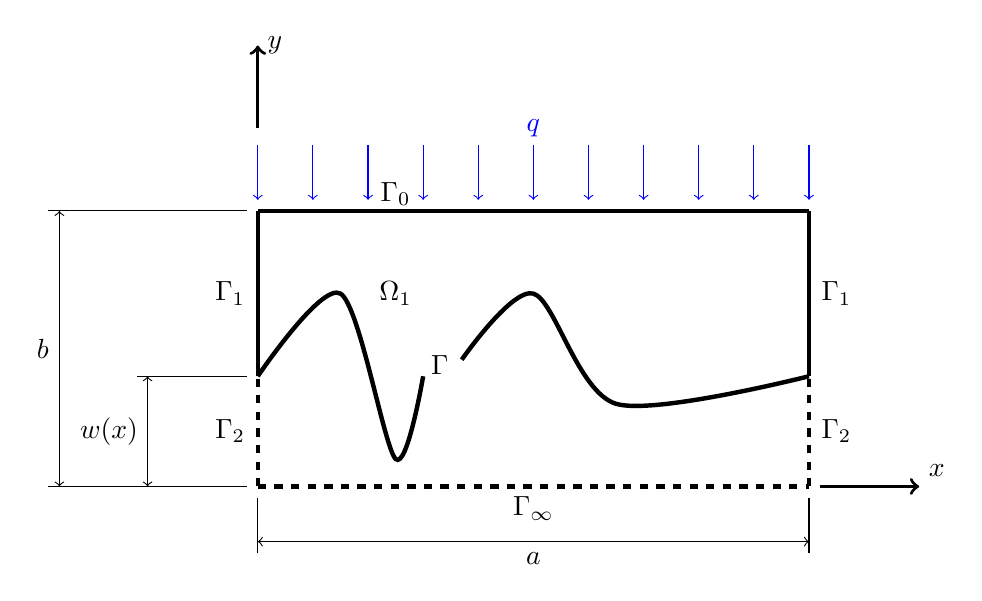
\begin{tikzpicture}[scale=0.7]
		
		\draw [ultra thick, dashed] (0, 0) -- (10, 0);
		%\draw [ultra thick] (0, 2) -- (7, 2);
		%\draw [ultra thick] (8, 2) -- (10, 2);
		\draw [ultra thick] plot [smooth] coordinates {(0, 2) (1.5, 3.5) (2.5, 0.5) (3, 2)};
		\draw [ultra thick] plot [smooth] coordinates {(3.7, 2.3) (5, 3.5) (6.5, 1.5) (10, 2)};
		\draw [ultra thick] (0, 5) -- (10, 5);
		\draw [ultra thick, dashed] (0, 0) -- (0, 2);	
		\draw [ultra thick] (0, 2) -- (0, 5);	
		\draw [ultra thick, dashed] (10, 0) -- (10, 2);
		\draw [ultra thick] (10, 2) -- (10, 5);
		
		\draw (2.5, 3.5) node {$\Omega_1$};
		\draw (3.3, 2.2) node {$\Gamma$};
		\draw (-0.5, 3.5) node {$\Gamma_1$};
		\draw (-0.5, 1) node {$\Gamma_2$};
		\draw (10.5, 3.5) node {$\Gamma_1$};
		\draw (10.5, 1) node {$\Gamma_2$};
		\draw (5, -0.4) node {$\Gamma_\infty$};
		\draw (2.5, 5.3) node {$\Gamma_0$};
		\draw [blue](5, 6.5) node {$q$};
		\draw (5, -1.3) node {$a$};
		\draw (-3.9, 2.5) node {$b$};
		\draw (-2.7, 1) node {$w(x)$};
		
		\node [above right] at (12, 0) {$x$};
		\node [right] at (0, 8) {$y$};
		
		\draw [->, blue] (0, 6.2) -- (0, 5.2);
		\draw [->, blue] (1, 6.2) -- (1, 5.2);
		\draw [->, blue] (2, 6.2) -- (2, 5.2);
		\draw [->, blue] (3, 6.2) -- (3, 5.2);
		\draw [->, blue] (4, 6.2) -- (4, 5.2);
		\draw [->, blue] (5, 6.2) -- (5, 5.2);
		\draw [->, blue] (6, 6.2) -- (6, 5.2);
		\draw [->, blue] (7, 6.2) -- (7, 5.2);
		\draw [->, blue] (8, 6.2) -- (8, 5.2);
		\draw [->, blue] (9, 6.2) -- (9, 5.2);
		\draw [->, blue] (10, 6.2) -- (10, 5.2);
		
		\draw [->, very thick] (10.2,0) -- (12,0);
		\draw [->, very thick] (0, 6.5) -- (0,8);
		
		\draw [-] (0, -0.2) -- (0, -1.2);
		\draw [-] (10, -0.2) -- (10, -1.2);
		\draw [<->] (0, -1) -- (10, -1);
		
		\draw [-] (-0.2, 0) -- (-3.8, 0);
		\draw [-] (-0.2, 5) -- (-3.8, 5);
		\draw [-] (-0.2, 2) -- (-2.2, 2);
		\draw [<->] (-3.6, 0) -- (-3.6, 5);
		\draw [<->] (-2.0, 0) -- (-2.0, 2);
		
		\end{tikzpicture}
		\caption{Extensão do subdomínio $\Omega_1$ para as funções $F_{1, j}$ e $G_{1, j}$}
		\label{fig5}
	\end{center}
\end{figure}

\begin{figure}[H]
	\begin{center}
		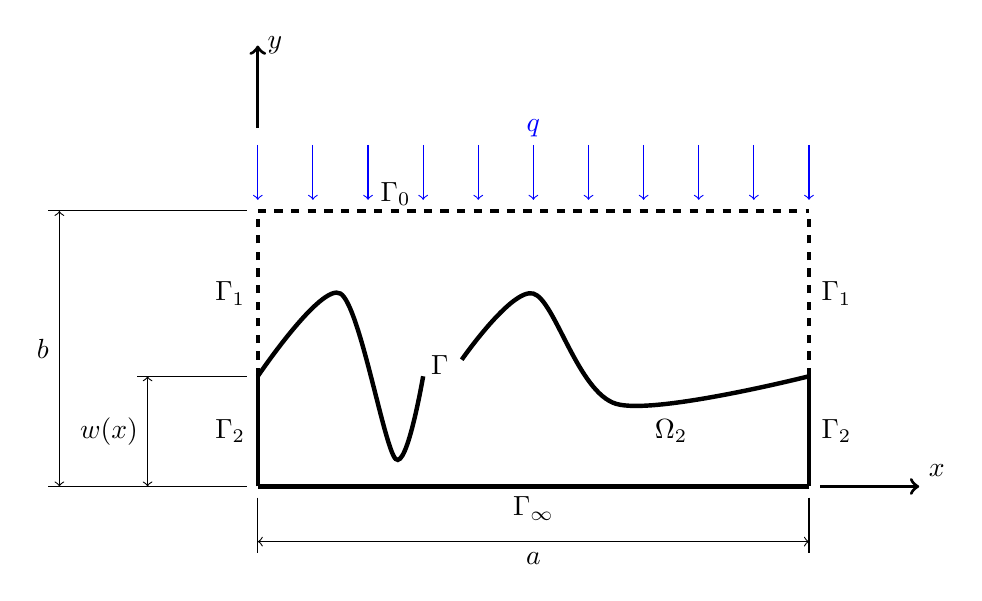
\begin{tikzpicture}[scale=0.7]
		
		\draw [ultra thick] (0, 0) -- (10, 0);
		%\draw [ultra thick] (0, 2) -- (7, 2);
		%\draw [ultra thick] (8, 2) -- (10, 2);
		\draw [ultra thick] plot [smooth] coordinates {(0, 2) (1.5, 3.5) (2.5, 0.5) (3, 2)};
		\draw [ultra thick] plot [smooth] coordinates {(3.7, 2.3) (5, 3.5) (6.5, 1.5) (10, 2)};
		\draw [ultra thick, dashed] (0, 5) -- (10, 5);
		\draw [ultra thick] (0, 0) -- (0, 2);	
		\draw [ultra thick, dashed] (0, 2) -- (0, 5);	
		\draw [ultra thick] (10, 0) -- (10, 2);
		\draw [ultra thick, dashed] (10, 2) -- (10, 5);
		
		\draw (7.5, 1) node {$\Omega_2$};	
		\draw (3.3, 2.2) node {$\Gamma$};
		\draw (-0.5, 3.5) node {$\Gamma_1$};
		\draw (-0.5, 1) node {$\Gamma_2$};
		\draw (10.5, 3.5) node {$\Gamma_1$};
		\draw (10.5, 1) node {$\Gamma_2$};
		\draw (5, -0.4) node {$\Gamma_\infty$};
		\draw (2.5, 5.3) node {$\Gamma_0$};
		\draw [blue](5, 6.5) node {$q$};
		\draw (5, -1.3) node {$a$};
		\draw (-3.9, 2.5) node {$b$};
		\draw (-2.7, 1) node {$w(x)$};
		
		\node [above right] at (12, 0) {$x$};
		\node [right] at (0, 8) {$y$};
		
		\draw [->, blue] (0, 6.2) -- (0, 5.2);
		\draw [->, blue] (1, 6.2) -- (1, 5.2);
		\draw [->, blue] (2, 6.2) -- (2, 5.2);
		\draw [->, blue] (3, 6.2) -- (3, 5.2);
		\draw [->, blue] (4, 6.2) -- (4, 5.2);
		\draw [->, blue] (5, 6.2) -- (5, 5.2);
		\draw [->, blue] (6, 6.2) -- (6, 5.2);
		\draw [->, blue] (7, 6.2) -- (7, 5.2);
		\draw [->, blue] (8, 6.2) -- (8, 5.2);
		\draw [->, blue] (9, 6.2) -- (9, 5.2);
		\draw [->, blue] (10, 6.2) -- (10, 5.2);
		
		\draw [->, very thick] (10.2,0) -- (12,0);
		\draw [->, very thick] (0, 6.5) -- (0,8);
		
		\draw [-] (0, -0.2) -- (0, -1.2);
		\draw [-] (10, -0.2) -- (10, -1.2);
		\draw [<->] (0, -1) -- (10, -1);
		
		\draw [-] (-0.2, 0) -- (-3.8, 0);
		\draw [-] (-0.2, 5) -- (-3.8, 5);
		\draw [-] (-0.2, 2) -- (-2.2, 2);
		\draw [<->] (-3.6, 0) -- (-3.6, 5);
		\draw [<->] (-2.0, 0) -- (-2.0, 2);
		
		\end{tikzpicture}
		\caption{Extensão do subdomínio $\Omega_2$ para as funções $F_{2, j}$}
		\label{fig6}
	\end{center}
\end{figure}

\subsection{Solução analítica dos problemas auxiliares através da Técnica da Transformada Integral Clássica}

\subsubsection{Problema homogêneo de autovalor associado ao primeiro problema auxiliar}

As condições de contorno \eqref{funcao_F_cc_T1_1a_cart} e \eqref{funcao_F_cc_T1_1b_cart}, na direção $x$, referentes ao problema de valor de contorno das funções $F_{1, j}$, são homogêneas e de segundo tipo. O
mesmo pode ser observado nas condições de contorno \eqref{funcao_F_cc_T1_3a_cart} e \eqref{funcao_F_cc_T1_3b_cart}, na direção $x$, referentes ao problema de valor de contorno das funções $F_{2, j}$.
Assim, o problema de autovalor associado, ou de Sturm-Liouville, será o mesmo para os dois problemas auxiliares:
\begin{subequations}
	\begin{alignat}{2}
	& \frac{d^2 X(\mu_m, x)}{d x^2} + \mu_m^2 X(\mu_m, x) = 0 \quad\quad\quad\quad\quad\quad && 0 < x < a \label{problema_vc_1a} \\ \nonumber \\
	& \frac{d X(\mu_m, x)}{d x} = 0 && x = 0 \label{problema_vc_1b} \\ \nonumber \\
	& \frac{d X(\mu_m, x)}{d x} = 0 && x = a \label{problema_vc_1c}
	\end{alignat}
\end{subequations}
onde $\mu_m$ são os autovalores e $X(\mu_m, x)$ são as autofunções correspondentes. Resolvendo-se o problema de autovalor definido em \eqref{problema_vc_1a}--\eqref{problema_vc_1c}, obtém-se \citep{livro_ozisik}:
\begin{align}
& X(\mu_m, x) = \left\lbrace
\begin{array}{ll}
1, & m = 0 \\ \\
\cos \mu_m x, & m = 1,2,3,\ldots
\end{array}
\right . \label{definicao_das_autofuncoes} \\ \nonumber \\
& N(\mu_m) = \left\lbrace
\begin{array}{ll}
a, \quad\quad\quad\quad & m = 0 \\ \\
\displaystyle\frac{a}{2}, & m = 1,2,3,\ldots
\end{array}
\right. \label{valor_integral_norm}
\end{align}
onde $N(\mu_m)$ é denominada integral de normalização, definida por
\begin{align}
N(\mu_m) = \int_0^a X(\mu_m, x)^2 dx
\end{align}

Os autovalores $\mu_m$ são dados por:
\begin{align}
\mu_m = \left\lbrace
\begin{array}{ll}
0, \quad\quad\quad\quad & m = 0 \\ \\
\displaystyle\frac{m\pi}{a}, & m = 1,2,3,\ldots
\end{array}
\right.
\end{align}

As autofunções $X(\mu_m, x), m=0,1,2,3,\ldots$, do problema de autovalor \eqref{problema_vc_1a}--\eqref{problema_vc_1c}, atendem à condição de ortogonalidade:
\begin{align}
& \int_0^a X(\mu_m, x)X(\mu_n, x)dx 
= \left\lbrace
\begin{array}{ll}
0 \quad\quad\quad\quad & \text{para  } m \neq n \\ \\
N(\mu_m) & \text{para  }m = n
\end{array}
\right. \label{ortogon}
\end{align}

\subsubsection{Definição do par transformada-inversa associado ao primeiro problema auxiliar}

Considera-se agora que tanto $F_{1, j}$ quanto $F_{2, j}$ possam ser representados em termos das autofunções $X(\mu_m, x)$ como segue:
\begin{align}
& F_{1, j}(x, y) = \sum_{m=0}^\infty C_{j,m}(y)X(\mu_m, x) \label{expansao_para_F1}\\ \nonumber \\
& F_{2, j}(x, y) = \sum_{m=0}^\infty D_{j,m}(y)X(\mu_m, x) \label{expansao_para_F2}
\end{align}

Os coeficientes $C_{j,m}(y)$ e $D_{j,m}(y)$ podem ser determinados através da aplicação da propriedade de ortogonalidade expressa em \eqref{ortogon}. Assim, multiplicando as equações
\eqref{expansao_para_F1} e \eqref{expansao_para_F2} por $X(\mu_n, x)$ e integrando em relação a $x$ no intervalo $0 < x < a$, obtém-se:
\begin{align}
& \int_0^a F_{1, j}(x, y)X(\mu_n, x)dx = \sum_{m=0}^\infty C_{j,m}(y) \int_0^a X(\mu_m, x)X(\mu_n, x)dx \label{somatorio_para_F1}\\ \nonumber \\
& \int_0^a F_{2, j}(x, y)X(\mu_n, x)dx = \sum_{m=0}^\infty D_{j,m}(y) \int_0^a X(\mu_m, x)X(\mu_n, x)dx \label{somatorio_para_F2}
\end{align}

As integrais acima, de acordo com a propriedade de ortogonalidade, anulam-se quando $m \ne n$, e são iguais a $N(\mu_m)$ quando $m = n$. Assim, cada somatório se reduz apenas ao
termo de índice $m$, de modo que os coeficientes serão dados por:
\begin{align}
& C_{j,m}(y) = \frac{1}{N(\mu_m)}\int_0^a F_{1, j}(x, y)X(\mu_m, x)dx \label{coef_para_F1}\\ \nonumber \\
& D_{j,m}(y) = \frac{1}{N(\mu_m)}\int_0^a F_{2, j}(x, y)X(\mu_m, x)dx \label{coef_para_F2}
\end{align}

Substituindo as relações \eqref{coef_para_F1} e \eqref{coef_para_F2} nos somatórios \eqref{expansao_para_F1} e \eqref{expansao_para_F2}, respectivamente, obtém-se:
\begin{align}
& F_{1, j}(x, y) = \sum_{m=0}^\infty \frac{X(\mu_m, x)}{N(\mu_m)}\int_0^a F_{1, j}(x', y)X(\mu_m, x')dx' \label{expansao_para_F1_nova}\\ \nonumber \\
& F_{2, j}(x, y) = \sum_{m=0}^\infty \frac{X(\mu_m, x)}{N(\mu_m)}\int_0^a F_{2, j}(x', y)X(\mu_m, x')dx' \label{expansao_para_F2_nova}
\end{align}

Denota-se a \textit{transformada integral} de $F_{1, j}$ e $F_{2, j}$ na direção $x$ respectivamente por $\bar{F}_{1,j,m}(y)$ e $\bar{F}_{2,j,m}(y)$.
Desse modo, cada uma das expressões acima pode ser dividida em duas partes, definindo o par \textit{transformada-inversa} para as funções $F_{1,j}$ e $F_{2,j}$:
\begin{itemize}
	\item Funções $F_{1, j}$:
	\begin{fleqn}
		\begin{alignat}{2}
		& \text{Inversa:} && F_{1, j}(x, y) = \sum_{m=0}^\infty \frac{X(\mu_m, x)}{N(\mu_m)}\bar{F}_{1,j,m}(y) \label{definicao_da_transf_inv_F1} \\ \nonumber \\
		& \text{Transformada:} \quad\quad && \bar{F}_{1,j,m}(y) = \int_0^a F_{1, j}(x, y) X(\mu_m, x) dx \label{definicao_da_transf_F1}
		\end{alignat}
	\end{fleqn}
	\item Funções $F_{2, j}$:
	\begin{fleqn}
		\begin{alignat}{2}
		& \text{Inversa:} && F_{2, j}(x, y) = \sum_{m=0}^\infty \frac{X(\mu_m, x)}{N(\mu_m)}\bar{F}_{2,j,m}(y) \label{definicao_da_transf_inv_F2} \\ \nonumber \\
		& \text{Transformada:} \quad\quad && \bar{F}_{2,j,m}(y) = \int_0^a F_{2, j}(x, y) X(\mu_m, x) dx
		\label{definicao_da_transf_F2}
		\end{alignat}
	\end{fleqn}
\end{itemize}

\subsubsection{Aplicação da transformação integral às equações do primeiro problema auxiliar}\label{secao_reciprocidade_F}

Uma vez definidos os pares transformada-inversa para as funções $F_{1,j}$ e $F_{2,j}$, procede-se à transformação integral na direção $x$ das equações
diferenciais parciais \eqref{funcao_F_harm_T1_cart} e \eqref{funcao_F_harm_T2_cart}, obtendo-se equações diferenciais ordinárias em $y$ envolvendo
as funções transformadas $\bar{F}_{1,j,m}(y)$ e $\bar{F}_{2,j,m}(y)$. Este procedimento será realizado inicialmente para a equação \eqref{funcao_F_harm_T1_cart};
os resultados serão análogos para a equação \eqref{funcao_F_harm_T2_cart}.

Multiplicando-se então a equação \eqref{funcao_F_harm_T1_cart} por $X(\mu_m, x)$ e integrando em relação a $x$ no intervalo $0 < x < a$, obtemos: 
\begin{align}
& \int_0^a  \frac{\partial^2 F_{1,j}(x, y)}{\partial x^2}X(\mu_m, x)dx + \int_0^a \frac{\partial^2 F_{1,j}(x, y)}{\partial y^2}X(\mu_m, x)dx = 0 
\end{align}

Na expressão acima, a primeira integral pode ser desenvolvida através de integração por partes, enquanto que na segunda integral, os operadores de derivada
em relação a $y$ e integração em relação a $x$ podem ser permutados:
\begin{align}
& \left[ \frac{\partial F_{1,j}(x, y)}{\partial x}X(\mu_m, x) \right]_0^a
-
\int_0^a  \frac{\partial F_{1,j}(x, y)}{\partial x}\frac{dX(\mu_m, x)}{dx} dx + \nonumber \\
& \frac{d^2}{d y^2}\int_0^a F_{1,j}(x, y)X(\mu_m, x)dx = 0 \nonumber \\ 
\Rightarrow & \frac{\partial F_{1,j}(a, y)}{\partial x}X(\mu_m, a) - \frac{\partial F_{1,j}(0, y)}{\partial x}X(\mu_m, 0)
-
\int_0^a  \frac{\partial F_{1,j}(x, y)}{\partial x}\frac{dX(\mu_m, x)}{dx} dx + \nonumber \\
& \frac{d^2}{d y^2}\int_0^a F_{1,j}(x, y)X(\mu_m, x)dx = 0
\end{align}

As condições de contorno \eqref{funcao_F_cc_T1_1a_cart} e \eqref{funcao_F_cc_T1_1b_cart} anulam os dois primeiros termos da expressão acima. A primeira
integral também pode ser desenvolvida por partes. A segunda integral é exatamente a transformada integral da função $F_{1, j}$, conforme a equação \eqref{definicao_da_transf_F1}.
Assim:
\begin{align}
&
- \left[ F_{1,j}(x, y)\frac{dX(\mu_m, x)}{dx} \right]_0^a
+ \int_0^a  F_{1,j}(x, y)\frac{d^2X(\mu_m, x)}{dx^2} dx + \frac{d^2 \bar{F}_{1,j,m}(y)}{d y^2} = 0 \nonumber \\
\Rightarrow &
- F_{1,j}(a, y)\frac{dX(\mu_m, a)}{dx}+ F_{1,j}(0, y)\frac{dX(\mu_m, 0)}{dx} + \int_0^a  F_{1,j}(x, y)\frac{d^2X(\mu_m, x)}{dx^2} dx + \nonumber \\
& \frac{d^2 \bar{F}_{1,j,m}(y)}{d y^2} = 0
\end{align}

Aplicando as condições de contorno \eqref{problema_vc_1b} e \eqref{problema_vc_1c}, a expressão resulta em: 
\begin{align}
&
\int_0^a  F_{1,j}(x, y)\frac{d^2X(\mu_m, x)}{dx^2} dx + \frac{d^2 \bar{F}_{1,j,m}(y)}{d y^2} = 0 \label{equacao_intermediaria_F1}
\end{align}

Da equação do problema homogêneo de autovalor associado \eqref{problema_vc_1a}, obtém-se:
\begin{align}
\frac{d^2 X(\mu_m, x)}{d x^2} = -\mu_m^2 X(\mu_m, x) \label{substituicao_autofuncao}
\end{align}

A substituição de \eqref{substituicao_autofuncao} em \eqref{equacao_intermediaria_F1} resulta em:
\begin{align}
&
\int_0^a  F_{1,j}(x, y)[-\mu_m^2 X(\mu_m, x)] dx + \frac{\partial^2 \bar{F}_{1,j,m}(y)}{\partial y^2} = 0 \nonumber \\
\Rightarrow &
\frac{d^2 \bar{F}_{1,j,m}(y)}{d y^2}
-
\mu_m^2 \int_0^a  F_{1,j}(x, y)X(\mu_m, x) dx = 0
\end{align}

Finalmente, aplicando a definição da transformada integral de $F_{1, j}$, obtém-se uma equação diferencial ordinária para $\bar{F}_{1,j,m}(y)$:
\begin{align}
\frac{d^2 \bar{F}_{1,j,m}(y)}{d y^2}
-
\mu_m^2 \bar{F}_{1,j,m}(y) = 0 \label{eq_dif_ord_F1}
\end{align}

Seguindo o mesmo procedimento para a equação \eqref{funcao_F_harm_T2_cart}, obtém-se uma equação diferencial ordinária para $\bar{F}_{2,j,m}(y)$:
\begin{align}
\frac{d^2 \bar{F}_{2,j,m}(y)}{d y^2}
-
\mu_m^2 \bar{F}_{2,j,m}(y) = 0 \label{eq_dif_ord_F2}
\end{align}

Neste ponto justifica-se o emprego do recurso da extensão de domínio (cf. secão \ref{secao_formulacao_aux}): a aplicação da transformação integral em $x$ às equações diferenciais parciais originais do problema eliminou a dependência em $x$, fornecendo assim as equações diferenciais ordinárias \eqref{eq_dif_ord_F1} e \eqref{eq_dif_ord_F2}, dependentes apenas de $y$. Se estas equações fossem resolvidas respectivamente para os domínios $w(x) < y < b$ e $0 < y < w(x)$, a variável $x$ seria reintroduzida, trazendo dificuldades na busca da solução, o que não acontece quando se adota o domínio $0 < y < b$ para resolução de ambas as equações. Nessas condições, as equações diferenciais \eqref{eq_dif_ord_F1} e \eqref{eq_dif_ord_F2} admitem as seguintes soluções fundamentais \citep{livro_boyce}:
\begin{align}
& f_{1,j,m}(y) = \sinh\mu_m y \label{basic_1}\\ \nonumber \\
& g_{1,j,m}(y) = \cosh\mu_m y \label{basic_2}
\end{align}

As soluções gerais das equações \eqref{eq_dif_ord_F1} e \eqref{eq_dif_ord_F2} serão então dadas pela combinação linear destas funções, que podem ser escritas na forma:
\begin{align}
& \bar{F}_{1,j,m}(y) = \mathbb{A}_{j,m}\frac{\sinh\mu_m (b - y)}{\sinh\mu_m b} + \mathbb{B}_{j,m}\frac{\sinh\mu_m y}{\sinh\mu_m b} \label{solucao_temporaria_F1}\\ \nonumber \\
& \bar{F}_{2,j,m}(y) = \mathbb{C}_{j,m}\frac{\sinh\mu_m (b - y)}{\sinh\mu_m b} + \mathbb{D}_{j,m}\frac{\sinh\mu_m y}{\sinh\mu_m b} \label{solucao_temporaria_F2}
\end{align} 
onde $\mathbb{A}_{j,m}, \mathbb{B}_{j,m}, \mathbb{C}_{j,m}$ e $\mathbb{D}_{j,m}$ são constantes a determinar\footnote{A expressão \eqref{solucao_temporaria_F1}, através da expansão dos argumentos das funções hiberbólicas, pode ser reescrita como:
	
	\begin{align*}
	& \bar{F}_{1,j,m}(y) = \left( \frac{\mathbb{B}_{j,m} - \mathbb{A}_{j,m} \cosh\mu_m b}{\sinh\mu_m b}\right)\sinh\mu_m y + \frac{\mathbb{A}_{j,m}\sinh\mu_m b}{\sinh\mu_m b}\cosh\mu_m y
	\end{align*}	
	que é uma combinação linear das soluções \eqref{basic_1} e \eqref{basic_2}; observações semelhantes podem ser feitas para a expressões \eqref{solucao_temporaria_F2}, \eqref{solucao_temporaria_F1_0} e \eqref{solucao_temporaria_F2_0}. Essa forma de expressar as soluções facilitará a determinação dos coeficientes $\mathbb{A}_{j,m}$, $\mathbb{B}_{j,m}$, $\mathbb{C}_{j,m}$ e $\mathbb{D}_{j,m}$, conforme será visto a seguir.
	
	}.
	
Aplicando-se a transformação integral às condições de contorno \eqref{funcao_F_cc_T1_2_cart} e \eqref{funcao_F_cc_T1_4_cart}, e substituindo as expressões \eqref{solucao_temporaria_F1} e \eqref{solucao_temporaria_F2}:

\begin{align}
& \int_0^a F_{1,j}(x, b)X(\mu_m, x)dx = \int_0^a \psi_j(x) X(\mu_m, x)dx \nonumber \\
& \Rightarrow \bar{F}_{1,j,m}(b) = \bar{\psi}_{j, m} \nonumber \\
& \Rightarrow \mathbb{A}_{j,m}\frac{\sinh 0}{\sinh\mu_m b} + \mathbb{B}_{j,m}\frac{\sinh \mu_m b}{\sinh\mu_m b} = \bar{\psi}_{j, m} \nonumber \\
& \Rightarrow \mathbb{B}_{j,m} = \bar{\psi}_{j, m} \label{resultado_cte_5}
\end{align} 

\begin{align}
& \int_0^a F_{2,j}(x, 0)X(\mu_m, x)dx = 0 \nonumber \\
& \Rightarrow \bar{F}_{2,j,m}(0) = 0 \nonumber \\
& \Rightarrow \mathbb{C}_{j,m}\frac{\sinh\mu_m b}{\sinh\mu_m b} + \mathbb{D}_{j,m}\frac{\sinh 0}{\sinh\mu_m b} = 0 \nonumber \\
& \Rightarrow \mathbb{C}_{j,m} = 0 \label{resultado_cte_8}
\end{align} 

Para o caso específico $\mu_0 = 0$, as equações diferenciais \eqref{eq_dif_ord_F1} e \eqref{eq_dif_ord_F2} admitem as seguintes soluções gerais:
\begin{align}
& \bar{F}_{1,j,0}(y) = \mathbb{A}_{j,0}\frac{b - y}{b} + \mathbb{B}_{j,0}\frac{y}{b} \label{solucao_temporaria_F1_0}\\ \nonumber \\
& \bar{F}_{2,j,0}(y) = \mathbb{C}_{j,0}\frac{b - y}{b} + \mathbb{D}_{j,0}\frac{y}{b} \label{solucao_temporaria_F2_0}
\end{align} 

Aplicando-se a transformação integral às condições de contorno \eqref{funcao_F_cc_T1_2_cart} e \eqref{funcao_F_cc_T1_4_cart} para $m = 0$, e substituindo as expressões \eqref{solucao_temporaria_F1_0} e \eqref{solucao_temporaria_F2_0}:
\begin{align}
& \int_0^a F_{1,j}(x, b)X(\mu_0, x)dx = \int_0^a \psi_j(x)X(\mu_0, x)dx \nonumber \\
& \Rightarrow \bar{F}_{1,j,0}(b) = \bar{\psi}_{j,0} \nonumber \\
& \Rightarrow \mathbb{A}_{j,0}\frac{0}{b} + \mathbb{B}_{j,0}\frac{b}{b} = \bar{\psi}_{j,0} \nonumber \\
& \Rightarrow \mathbb{B}_{j,0} = \bar{\psi}_{j,0} \label{resultado_cte_2}
\end{align} 

\begin{align}
& \int_0^a F_{2,j}(x, 0)X(\mu_0, x)dx = 0 \nonumber \\
& \Rightarrow \bar{F}_{2,j,0}(0) = 0 \nonumber \\
& \Rightarrow \mathbb{C}_{j,0}\frac{b}{b} + \mathbb{D}_{j,0}\frac{0}{b} = 0 \nonumber \\
& \therefore \mathbb{C}_{j,0} = 0 \label{resultado_cte_3}
\end{align}

Fazendo a substituição dos resultados encontrados para as constantes \eqref{resultado_cte_5} e \eqref{resultado_cte_8}
em \eqref{solucao_temporaria_F1} e \eqref{solucao_temporaria_F2}, obtém-se as expressões para as transformadas das funções $F_{1,j}$ e $F_{2,j}$:
\begin{align}
& \bar{F}_{1,j,m}(y) = \mathbb{A}_{j,m}\frac{\sinh\mu_m (b - y)}{\sinh\mu_m b} + \bar{\psi}_{j, m}\frac{\sinh\mu_m y}{\sinh\mu_m b} \label{math_A_1} \\ \nonumber \\
& \bar{F}_{2,j,m}(y) = \mathbb{D}_{j,m}\frac{\sinh\mu_m y}{\sinh\mu_m b} \label{math_A_2}
\end{align} 

Para o caso específico do autovalor nulo, associado às expressões \eqref{solucao_temporaria_F1_0} e \eqref{solucao_temporaria_F2_0}, a substituição dos
resultados encontrados em \eqref{resultado_cte_2} e \eqref{resultado_cte_3} fornece:
\begin{align}
& \bar{F}_{1,j,0}(y) = \mathbb{A}_{j,0}\frac{b - y}{b} + \bar{\psi}_{j,0}\frac{y}{b} \label{math_A_3} \\ \nonumber \\
& \bar{F}_{2,j,0}(y) = \mathbb{D}_{j,0}\frac{y}{b} \label{math_A_4}
\end{align} 

Substituindo esses resultados
nas expressões das inversas \eqref{definicao_da_transf_inv_F1} e \eqref{definicao_da_transf_inv_F2}, chega-se a:
\begin{align}
F_{1, j}(x, y) = & \frac{\mathbb{A}_{j,0}(b - y) + \bar{\psi}_{j,0}y}{ab} + \nonumber \\
&\frac{2}{a}\sum_{m=1}^\infty\left[\mathbb{A}_{j,m}\frac{\sinh\mu_m (b - y)}{\sinh\mu_m b} + \bar{\psi}_{j, m}\frac{\sinh\mu_m y}{\sinh\mu_m b}\right]\cos\mu_m x
\label{solucao_transf_inversa_F1_com_dependencia}
\end{align}
\begin{align}
F_{2, j}(x, y) = \mathbb{D}_{j,0}\frac{y}{ab}  + \frac{2}{a}\sum_{m=1}^\infty\mathbb{D}_{j,m}\frac{\sinh\mu_m y}{\sinh\mu_m b} \cos\mu_m x
\label{solucao_transf_inversa_F2_com_dependencia}
\end{align}

As constantes $\mathbb{A}_{j,m}$ e $\mathbb{D}_{j,m}$ serão levantadas através da substituição das soluções analíticas de $F_{1,j}$ e $F_{2,j}$, expressas nas equações \eqref{definicao_da_transf_inv_F1} e
\eqref{definicao_da_transf_inv_F2}, nas condições de contorno \eqref{funcao_F_cc_grad_T1_cart} e \eqref{funcao_F_cc_T1_5_cart}, com posterior aplicação da transformação integral às equações resultantes, levando a um sistema de equações lineares.

Assim, fazendo esta
substituição para a equação \eqref{funcao_F_cc_grad_T1_cart}, obtém-se:
\begin{align}
& F_{1,j}(x, w(x)) = F_{2, j}(x, w(x)) \nonumber \\
& \Rightarrow \sum_{m=0}^M \frac{X_m(x)}{N(\mu_m)}\bar{F}_{1,j,m}(w(x)) = \sum_{m=0}^\infty \frac{X_m(x)}{N(\mu_m)}\bar{F}_{2,j,m}(w(x))
\end{align}
onde $X_m(x) \equiv X(\mu_m, x)$.

Uma vez que os termos de índice $m = 0$ precisam de um tratamento especial, eles serão separados do somatório principal:
\begin{align}
& \frac{X_0(x)}{N(\mu_0)}\bar{F}_{1,j,0}(w(x)) +
\sum_{m=1}^\infty \frac{X_m(x)}{N(\mu_m)}\bar{F}_{1,j,m}(w(x))
= \nonumber \\
& \frac{X_0(x)}{N(\mu_0)}\bar{F}_{2,j,0}(w(x)) +
\sum_{m=1}^\infty \frac{X_m(x)}{N(\mu_m)}\bar{F}_{2,j,m}(w(x))
\end{align}

Substituindo pelos resultados em \eqref{math_A_1}, \eqref{math_A_2}, \eqref{math_A_3} e \eqref{math_A_4}:
\begin{align}
& \frac{1}{a}\left[\mathbb{A}_{j,0}\frac{b - w(x)}{b} + \bar{\psi}_{j,0}\frac{w(x)}{b}\right] + \nonumber \\
& \quad\quad
\sum_{m=1}^\infty \frac{2}{a}X_m(x)\left\lbrace\mathbb{A}_{j,m}\frac{\sinh\mu_m [b - w(x)]}{\sinh\mu_m b} + \bar{\psi}_{j, m}\frac{\sinh\mu_m w(x)}{\sinh\mu_m b}\right\rbrace
= \nonumber \\
& \quad\quad \frac{1}{a}\mathbb{D}_{j,0}\frac{w(x)}{b} + 
\sum_{m=1}^\infty \frac{2}{a}X_m(x)\mathbb{D}_{j,m}\frac{\sinh\mu_m w(x)}{\sinh\mu_m b} \nonumber \\
& \Rightarrow \mathbb{A}_{j,0}\frac{b - w(x)}{b} + \bar{\psi}_{j,0}\frac{w(x)}{b} + \nonumber \\
& \quad\quad
2 \sum_{m=1}^\infty \left\lbrace\mathbb{A}_{j,m}\frac{\sinh\mu_m [b - w(x)]}{\sinh\mu_m b} + \bar{\psi}_{j, m}\frac{\sinh\mu_m w(x)}{\sinh\mu_m b}\right\rbrace X_m(x)
= \nonumber \\
& \quad\quad \mathbb{D}_{j,0}\frac{w(x)}{b} +  
2 \sum_{m=1}^\infty \mathbb{D}_{j,m}\frac{\sinh\mu_m w(x)}{\sinh\mu_m b}X_m(x) \nonumber \\
& \Rightarrow \mathbb{A}_{j,0}\frac{b - w(x)}{b} + 
2 \sum_{m=1}^\infty \mathbb{A}_{j,m}\frac{\sinh\mu_m [b - w(x)]}{\sinh\mu_m b}X_m(x) - \nonumber \\
& \quad\quad   \mathbb{D}_{j,0}\frac{w(x)}{b} - 2 \sum_{m=1}^\infty \mathbb{D}_{j,m}\frac{\sinh\mu_m w(x)}{\sinh\mu_m b}X_m(x)
= \nonumber \\
& \quad\quad  
-
\bar{\psi}_{j,0}\frac{w(x)}{b}
-
2 \sum_{m=1}^\infty \bar{\psi}_{j, m}\frac{\sinh\mu_m w(x)}{\sinh\mu_m b}X_m(x)
\end{align}
ou, de forma compacta:
\begin{align}
\sum_{m = 0}^\infty a_m(x) \mathbb{A}_{j,m} + \sum_{m = 0}^\infty b_m(x) \mathbb{D}_{j,m} = c_{j}(x) \label{compacta_1}
\end{align}
onde
\begin{align}
& a_m(x) = \left\lbrace
\begin{array}{ll}
\displaystyle \frac{b - w(x)}{b}, & m = 0 \\ \\
\displaystyle 2 \frac{\sinh\mu_m [b - w(x)]}{\sinh\mu_m b}X_m(x) , & m \ne 0
\end{array}
\right. \\
& b_m(x) = \left\lbrace
\begin{array}{ll}
\displaystyle -\frac{w(x)}{b}, & m = 0 \\ \\
\displaystyle - 2 \frac{\sinh\mu_m w(x)}{\sinh\mu_m b} X_m(x), & m \ne 0
\end{array}
\right. \\
& c_{j}(x) = -
\bar{\psi}_{j,0}\frac{w(x)}{b}
-
2 \sum_{m=1}^\infty \bar{\psi}_{j, m}\frac{\sinh\mu_m w(x)}{\sinh\mu_m b}X_m(x)
\end{align}

Fazendo agora a
substituição de \eqref{definicao_da_transf_inv_F1} e
\eqref{definicao_da_transf_inv_F2} na equação \eqref{funcao_F_cc_T1_5_cart}, obtém-se:
\begin{align}
& k_2\left[w'(x)\frac{\partial F_{2,j}(x, w(x))}{\partial x} - \frac{\partial F_{2,j}(x, w(x))}{\partial y}\right] = \nonumber \\
& k_1\left[w'(x)\frac{\partial F_{1,j}(x, w(x))}{\partial x} - \frac{\partial F_{1,j}(x, w(x))}{\partial y}\right] \nonumber \\
& \Rightarrow k_2\left[w'(x)\sum_{m=0}^\infty \frac{X'_m(x)}{N(\mu_m)}\bar{F}_{2,j,m}(w(x)) - \sum_{m=0}^\infty \frac{X_m(x)}{N(\mu_m)}\bar{F}'_{2,j,m}(w(x)) \right] = \nonumber \\
& \quad\quad k_1\left[w'(x)\sum_{m=0}^\infty \frac{X'_m(x)}{N(\mu_m)}\bar{F}_{1,j,m}(w(x)) - \sum_{m=0}^\infty \frac{X_m(x)}{N(\mu_m)}\bar{F}'_{1,j,m}(w(x)) \right] \nonumber \\
& \Rightarrow  \sum_{m=0}^\infty \frac{k_2}{N(\mu_m)} \left[ w'(x) X'_m(x)\bar{F}_{2,j,m}(w(x)) - X_m(x)\bar{F}'_{2,j,m}(w(x)) \right] = \nonumber \\
& \quad\quad \sum_{m=0}^\infty \frac{k_1}{N(\mu_m)} \left[ w'(x) X'_m(x)\bar{F}_{1,j,m}(w(x)) - X_m(x)\bar{F}'_{1,j,m}(w(x)) \right]
\end{align}

Separando os termos $m = 0$ do restante do somatório:
\begin{align}
& \frac{k_2}{N(\mu_0)} \left[ w'(x) \cancelto{0}{X'_0(x)}\bar{F}_{2,j,0}(w(x)) -  X_0(x)\bar{F}'_{2,j,0}(w(x)) \right] + \nonumber \\
& \sum_{m=1}^\infty \frac{k_2}{N(\mu_m)} \left[ w'(x) X'_m(x)\bar{F}_{2,j,m}(w(x)) - X_m(x)\bar{F}'_{2,j,m}(w(x)) \right] = \nonumber \\
& \frac{k_1}{N(\mu_0)} \left[w'(x) \cancelto{0}{X'_0(x)}\bar{F}_{1,j,0}(w(x)) - X_0(x)\bar{F}'_{1,j,0}(w(x)) \right] + \nonumber \\
& \sum_{m=1}^\infty \frac{k_1}{N(\mu_m)} \left[w'(x) X'_m(x)\bar{F}_{1,j,m}(w(x)) - X_m(x)\bar{F}'_{1,j,m}(w(x)) \right]
\end{align}

Substituindo pelos resultados em \eqref{math_A_1}, \eqref{math_A_2}, \eqref{math_A_3} e \eqref{math_A_4}:
\begin{align}
& \frac{k_2}{a} \left( -  \frac{\mathbb{D}_{j,0}}{b} \right) + \nonumber \\
& \quad\quad \sum_{m=1}^\infty \frac{2k_2}{a} \left[\mathbb{D}_{j,m} w'(x) \frac{\sinh\mu_m w(x)}{\sinh\mu_m b}  X'_m(x) - \mu_m\mathbb{D}_{j,m}\frac{\cosh\mu_m w(x)}{\sinh\mu_m b} X_m(x) \right] = \nonumber \\
& \quad\quad \frac{k_1}{a} \left( - \frac{\bar{\psi}_{j,0} - \mathbb{A}_{j,0}}{b} \right) + \nonumber \\
& \quad\quad \sum_{m=1}^\infty \frac{2k_1}{a} \Bigg\{\mathbb{A}_{j,m}w'(x)\frac{\sinh\mu_m [b - w(x)]}{\sinh\mu_m b}X'_m(x) + \bar{\psi}_{j, m}w'(x)\frac{\sinh\mu_m w(x)}{\sinh\mu_m b}X'_m(x) + \nonumber \\
& \quad\quad \mu_m\mathbb{A}_{j,m}\frac{\cosh\mu_m [b - w(x)]}{\sinh\mu_m b}X_m(x) - \mu_m\bar{\psi}_{j, m}\frac{\cosh\mu_m w(x)}{\sinh\mu_m b}X_m(x) \Bigg\} \nonumber \\
%
& \Rightarrow 
-  \frac{k_1}{b}\mathbb{A}_{j,0} - \nonumber \\
& \quad\quad 2k_1 \sum_{m=1}^\infty \mathbb{A}_{j,m} \left\lbrace w'(x)\frac{\sinh\mu_m [b - w(x)]}{\sinh\mu_m b}X'_m(x) +   \mu_m\frac{\cosh\mu_m [b - w(x)]}{\sinh\mu_m b}X_m(x)\right\rbrace - \nonumber \\
&  \quad\quad \frac{k_2}{b}\mathbb{D}_{j,0} + \nonumber \\
& \quad\quad 2k_2\sum_{m=1}^\infty  \mathbb{D}_{j,m}\left[ w'(x) \frac{\sinh\mu_m w(x)}{\sinh\mu_m b}  X'_m(x) - \mu_m\frac{\cosh\mu_m w(x)}{\sinh\mu_m b} X_m(x) \right]  = \nonumber \\
& \quad\quad -\frac{k_1}{b}\bar{\psi}_{j,0} + \nonumber \\
& \quad\quad  2k_1 \sum_{m=1}^\infty \bar{\psi}_{j, m}\left[ w'(x)\frac{\sinh\mu_m w(x)}{\sinh\mu_m b}X'_m(x) -  \mu_m\frac{\cosh\mu_m w(x)}{\sinh\mu_m b}X_m(x)\right]
\end{align}

ou, de forma compacta:
\begin{align}
\sum_{m = 0}^\infty p_m(x) \mathbb{A}_{j,m} + \sum_{m = 0}^\infty q_m(x) \mathbb{D}_{j,m} = r_{j}(x) \label{compacta_2}
\end{align}
onde
\begin{align}
& p_m(x) = \left\lbrace
\begin{array}{ll}
\displaystyle -\frac{k_1}{b}, & m = 0 \\ \\
\displaystyle -2k_1\left\lbrace w'(x)\frac{\sinh\mu_m [b - w(x)]}{\sinh\mu_m b}X'_m(x) +   \mu_m\frac{\cosh\mu_m [b - w(x)]}{\sinh\mu_m b}X_m(x)\right\rbrace, & m \ne 0
\end{array}
\right. \label{compacta_p} \\
& q_m(x) = \left\lbrace
\begin{array}{ll}
\displaystyle -\frac{k_2}{b}, & m = 0 \\ \\
\displaystyle 2k_2\left[ w'(x) \frac{\sinh\mu_m w(x)}{\sinh\mu_m b}  X'_m(x) - \mu_m\frac{\cosh\mu_m w(x)}{\sinh\mu_m b} X_m(x) \right], & m \ne 0
\end{array}
\right. \label{compacta_q} \\
&
r_{j}(x) = -\frac{k_1}{b}\bar{\psi}_{j,0} + \nonumber \\
& \quad\quad  2k_1 \sum_{m=1}^\infty \bar{\psi}_{j, m}\left[ w'(x)\frac{\sinh\mu_m w(x)}{\sinh\mu_m b}X'_m(x) -  \mu_m\frac{\cosh\mu_m w(x)}{\sinh\mu_m b}X_m(x)\right] \label{compacta_r}
\end{align}

As expressões \eqref{compacta_1} e \eqref{compacta_2} definem um sistema infinito de equações lineares cujos coeficientes são termos
dependentes da variável $x$. A fim de determinar os valores de $\mathbb{A}_{j,m}$ e $\mathbb{D}_{j,m}$ que satisfazem este sistema, o mesmo
deve ser truncado até uma quantidade finita de termos representada por $M$, de modo que cada igualdade será susbtituída por uma aproximação:
\begin{align}
& \sum_{m = 0}^M a_m(x) \mathbb{A}_{j,m} + \sum_{m = 0}^M b_m(x) \mathbb{D}_{j,m} \approx c_{j}(x) \label{compacta_aprox_1} \\
& \sum_{m = 0}^M p_m(x) \mathbb{A}_{j,m} + \sum_{m = 0}^M q_m(x) \mathbb{D}_{j,m} \approx r_{j}(x) \label{compacta_aprox_2}
\end{align}

As relações \eqref{compacta_aprox_1} e \eqref{compacta_aprox_2} são válidas para todo o domínio contínuo $0 \le x \le a$, e são funções apenas de $x$. Para eliminar a dependência com a variável $x$, pode-se aplicar a transformação integral nessas equações:
\begin{align}
& \sum_{m = 0}^M \mathbb{A}_{j,m}\int_0^a a_m(x)X(\mu_n, x)dx + \sum_{m = 0}^M \mathbb{D}_{j,m} \int_0^a b_m(x)X(\mu_n, x)dx \approx \nonumber \\ 
& \quad\quad\quad\quad\int_0^a c_{j}(x)X(\mu_n, x)dx \label{compacta_aprox_1_integr}
\end{align}
\begin{align}
& \sum_{m = 0}^M \mathbb{A}_{j,m}\int_0^a p_m(x)X(\mu_n, x)dx + \sum_{m = 0}^M \mathbb{D}_{j,m} \int_0^a q_m(x)X(\mu_n, x)dx \approx \nonumber \\ 
& \quad\quad\quad\quad\int_0^a r_{j}(x)X(\mu_n, x)dx  \label{compacta_aprox_2_integr}
\end{align}
ou
\begin{align}
& \sum_{m = 0}^M \bar{a}_{n,m} \mathbb{A}_{j,m} + \sum_{m = 0}^M \bar{b}_{n,m} \mathbb{D}_{j,m} \approx \bar{c}_{n,j} \label{sistema_para_coeficientes_1}
\\
& \sum_{m = 0}^M \bar{p}_{n,m} \mathbb{A}_{j,m} + \sum_{m = 0}^M \bar{q}_{n,m} \mathbb{D}_{j,m} \approx \bar{r}_{n,,j} \label{sistema_para_coeficientes_2}
\end{align}
onde adotou-se a susbtituição $\bar{\sigma}_{n,m} = \displaystyle \int_0^a \sigma_m(x)X(\mu_n, x)dx$.
\\

As equações \eqref{sistema_para_coeficientes_1} e \eqref{sistema_para_coeficientes_2} podem ser reescritas na forma matricial:
\begin{align}
\mathbf{M}\mathbf{\xi} \approx \mathbf{b} \label{sistema_para_coeficientes_3}
\end{align}
onde
\begin{align}
\mathbf{M} =
\begin{bmatrix}
\bar{a}_{0,0} & \bar{b}_{0,0} & \bar{a}_{0,1} & \bar{b}_{0,1} &  \ldots & \bar{a}_{0,M} & \bar{b}_{0,M} \\
\bar{p}_{0,0} & \bar{q}_{0,0} & \bar{p}_{0,1} & \bar{q}_{0,1} &  \ldots & \bar{p}_{0,M} & \bar{q}_{0,M} \\
\bar{a}_{1,0} & \bar{b}_{1,0} & \bar{a}_{1,1} & \bar{b}_{1,1} &  \ldots & \bar{a}_{1,M} & \bar{b}_{1,M} \\
\bar{p}_{1,0} & \bar{q}_{1,0} & \bar{p}_{1,1} & \bar{q}_{1,1} &  \ldots & \bar{p}_{1,M} & \bar{q}_{1,M} \\
\bar{a}_{2,0} & \bar{b}_{2,0} & \bar{a}_{2,1} & \bar{b}_{2,1} &  \ldots & \bar{a}_{2,M} & \bar{b}_{2,M} \\
\bar{p}_{2,0} & \bar{q}_{2,0} & \bar{p}_{2,1} & \bar{q}_{2,1} &  \ldots & \bar{p}_{2,M} & \bar{q}_{2,M} \\
\ldots & \ldots & \ldots & \ldots & \ddots & \ldots & \ldots\\
\bar{a}_{M,0} & \bar{b}_{M,0} & \bar{a}_{M,1} & \bar{b}_{M,1} &  \ldots & \bar{a}_{M,M} & \bar{b}_{M,M} \\
\bar{p}_{M,0} & \bar{q}_{M,0} & \bar{p}_{M,1} & \bar{q}_{M,1} &  \ldots & \bar{p}_{M,M} & \bar{q}_{M,M}
\end{bmatrix}
\end{align}

\begin{align}
\mathbf{\xi}
=
\begin{bmatrix}
\mathbb{A}_{0,0} & \mathbb{A}_{1,0} & \mathbb{A}_{2,0} & \ldots & \mathbb{A}_{N,0} \\
\mathbb{D}_{0,0} & \mathbb{D}_{1,0} & \mathbb{D}_{2,0} & \ldots & \mathbb{D}_{N,0} \\
\mathbb{A}_{0,1} & \mathbb{A}_{1,1} & \mathbb{D}_{2,1} & \ldots & \mathbb{A}_{N,1} \\
\mathbb{D}_{0,1} & \mathbb{D}_{1,1} & \mathbb{D}_{2,1} & \ldots & \mathbb{D}_{N,1} \\
\ldots & \ldots & \ldots & \ddots & \ldots \\
\mathbb{A}_{0,M} & \mathbb{A}_{1,M} & \mathbb{D}_{2,M} & \ldots & \mathbb{A}_{N,M} \\
\mathbb{D}_{0,M} & \mathbb{D}_{1,M} & \mathbb{D}_{2,M} & \ldots & \mathbb{D}_{N,M}
\end{bmatrix}
\end{align}

\begin{align}
\mathbf{b}
=
\begin{bmatrix}
\bar{c}_{0, 0} & \bar{c}_{0, 1} &\bar{c}_{0, 2} & \ldots & \bar{c}_{0, N} \\
\bar{r}_{0, 0} & \bar{r}_{0, 1} &\bar{r}_{0, 2} & \ldots & \bar{r}_{0, N} \\
\bar{c}_{1, 0} & \bar{c}_{1, 1} &\bar{c}_{1, 2} & \ldots & \bar{c}_{1, N} \\
\bar{r}_{1, 0} & \bar{r}_{1, 1} &\bar{r}_{1, 2} & \ldots & \bar{r}_{1, N} \\
\bar{c}_{2, 0} & \bar{c}_{2, 1} &\bar{c}_{2, 2} & \ldots & \bar{c}_{2, N} \\
\bar{r}_{2, 0} & \bar{r}_{2, 1} &\bar{r}_{2, 2} & \ldots & \bar{r}_{2, N} \\
\ldots & \ldots & \ldots & \ddots & \ldots \\
\bar{c}_{M, 0} & \bar{c}_{M, 1} &\bar{c}_{M, 2} & \ldots & \bar{c}_{M, N} \\
\bar{r}_{M, 0} & \bar{r}_{M, 1} &\bar{r}_{M, 2} & \ldots & \bar{r}_{M, N}
\end{bmatrix}
\label{sistema_para_coeficientes_3_end}
\end{align}

Uma vez conhecida a família de funções $\psi_j(x)$ (e consequentemente suas transformadas integrais $\bar{\psi}_{j, m}$), pode-se calcular os termos das matrizes $\mathbf{M}$ e $\mathbf{b}$ que compõem o sistema definido por \eqref{sistema_para_coeficientes_3}. Este sistema deve ser resolvido para cada coluna da matriz $\mathbf{b}$, e os coeficientes obtidos, ou seja, as colunas da matriz $\mathbf{\xi}$, são os que melhor representam as aproximações \eqref{compacta_aprox_1} e \eqref{compacta_aprox_2}. Assumindo então que esta aproximação é suficientemente satisfatória, o sinal de aproximação em \eqref{compacta_aprox_1} e \eqref{compacta_aprox_2}, e expressões análogas, será substituído pelo sinal de igual. Em tese, se o sistema infinito pudesse ser resolvido numericamente, as representações seriam dadas por \eqref{compacta_1} e \eqref{compacta_2} e seriam exatas.

%Aplicando a transformação integral às equações \eqref{compacta_1} e \eqref{compacta_2}:
%\begin{align}
%& \sum_{m = 0}^M \mathbb{A}_{j,m}\int_0^a a_m(x)X_n(x)dx + \sum_{m = 0}^M \mathbb{D}_{j,m}\int_0^a b_m(x)X_n(x)dx = \nonumber \\
%& \quad\quad \int_0^a c_{j}(x) X_n(x)dx \nonumber \\
%& \therefore 
%\sum_{m = 0}^M \bar{a}_{m, n} \mathbb{A}_{j,m} + \sum_{m = 0}^M \bar{b}_{m, n} \mathbb{D}_{j,m} = \bar{c}_{j, n}
%\label{sistema_para_coeficientes_1}
%\end{align}
%\begin{align}
%& \sum_{m = 0}^M \mathbb{A}_{j,m}\int_0^a p_m(x)X_n(x)dx + \sum_{m = 0}^M \mathbb{D}_{j,m}\int_0^a q_m(x)X_n(x)dx = \nonumber \\
%& \quad\quad \int_0^a r_{j}(x) X_n(x)dx \nonumber \\
%& \therefore 
%\sum_{m = 0}^M \bar{p}_{m, n} \mathbb{A}_{j,m} + \sum_{m = 0}^M \bar{q}_{m, n} \mathbb{D}_{j,m} = \bar{r}_{j, n}
%\label{sistema_para_coeficientes_2}
%\end{align}
%
%As equações \eqref{sistema_para_coeficientes_1} e \eqref{sistema_para_coeficientes_2} configuram um sistema de equações lineares cujas incógnitas são os termos $\mathbb{A}_{j,m}$ e $\mathbb{D}_{j,m}$.
%Assumindo que $\psi_j(x)$ já é conhecida (e consequentemente sua transformada $\bar{\psi}_{j, m}$), os coeficientes $\mathbb{A}_{j, m}$ e $\mathbb{D}_{j, m}$ podem
%ser obtidos através da solução deste sistema de equações lineares,
%e susbtituídas nas relações \eqref{solucao_transf_inversa_F1_com_dependencia} e \eqref{solucao_transf_inversa_F2_com_dependencia}, devidamente truncadas
%até o índice $M$:
%\begin{align}
%F_{1, j}(x, y) = & \frac{\mathbb{A}_{j,0}(b - y) + \bar{\psi}_{j,0}y}{ab} + \nonumber \\
%&\frac{2}{a}\sum_{m=1}^M \left[\mathbb{A}_{j,m}\frac{\sinh\mu_m (b - y)}{\sinh\mu_m b} + \bar{\psi}_{j, m}\frac{\sinh\mu_m y}{\sinh\mu_m b}\right]\cos\mu_m x
%\label{solucao_transf_inversa_F1_com_dependencia_truncado}
%\end{align}
%\begin{align}
%F_{2, j}(x, y) = \mathbb{D}_{j,0}\frac{y}{ab}  + \frac{2}{a}\sum_{m=1}^M \mathbb{D}_{j,m}\frac{\sinh\mu_m y}{\sinh\mu_m b} \cos\mu_m x
%\label{solucao_transf_inversa_F2_com_dependencia_truncado}
%\end{align}

Para obter a expressão analítica para a função $\beta_j$, aplica-se a definição da derivada direcional \eqref{derivada_direcional_para_n1} na definção de $\beta_j$ dada por \eqref{expressao_define_beta}, obtendo:
\begin{align}
\beta_j(x) = \frac{k_1}{\sqrt{1 + w'(x)^2}}\left[w'(x)\frac{\partial F_{1, j}(x, w(x))}{\partial x} - \frac{\partial F_{1, j}(x, w(x))}{\partial y}\right] \label{expansao_beta}
\end{align}

Calculando separadamente as derivadas parciais de $F_{1, j}$, a partir de \eqref{solucao_transf_inversa_F1_com_dependencia}, e truncando o somatório até o índice $M$:
\begin{align}
\frac{\partial F_{1, j}(x, y)}{\partial x} = & -\frac{2}{a}\sum_{m=1}^M \mu_m \left[\mathbb{A}_{j,m}\frac{\sinh\mu_m (b - y)}{\sinh\mu_m b} + \bar{\psi}_{j, m}\frac{\sinh\mu_m y}{\sinh\mu_m b}\right]\sin\mu_m x
\label{derivada_parcial_F1_x} \\
\frac{\partial F_{1, j}(x, y)}{\partial y} = & \frac{\bar{\psi}_{j,0} - \mathbb{A}_{j,0}}{ab} - \nonumber \\
&\frac{2}{a}\sum_{m=1}^M \mu_m \left[\mathbb{A}_{j,m}\frac{\cosh\mu_m (b - y)}{\sinh\mu_m b} - \bar{\psi}_{j, m}\frac{\cosh\mu_m y}{\sinh\mu_m b}\right]\cos\mu_m x
\label{derivada_parcial_F1_y}
\end{align}

Substituindo em \eqref{expansao_beta} as expressões \eqref{derivada_parcial_F1_x} e \eqref{derivada_parcial_F1_y} avaliadas em $y = w(x)$, obtém-se:
\begin{align}
\beta_j(x) = & \frac{k_1}{\sqrt{1 + w'(x)^2}}\left\lbrace \frac{\mathbb{A}_{j,0} - \bar{\psi}_{j,0}}{ab} \right.  + \nonumber \\
\frac{2}{a}\sum_{m=1}^M \mu_m & \left[ \mathbb{A}_{j,m}\frac{\cos\mu_m x\cosh\mu_m v(x) - w'(x)\sin\mu_m x\sinh\mu_m v(x)}{\sinh\mu_m b} \right. - \nonumber \\
&\left. \left. \bar{\psi}_{j, m}\frac{w'(x)\sin\mu_m x\sinh\mu_m w(x) + \cos\mu_m x\cosh\mu_m w(x)}{\sinh\mu_m b}\right] \right\rbrace
\label{serie_para_beta}
\end{align}
onde, por conveniência, fez-se $v(x) = b - w(x)$.



\subsubsection{Solução do segundo problema auxiliar}\label{secao_reciprocidade_G}

O segundo problema auxiliar, definido pelas equações \eqref{funcao_G_harm_T1_cart} a \eqref{funcao_G_cc_T1_1b_cart}, tem forma idêntica ao do problema formulado pelas equações \eqref{funcao_F_harm_T1_cart} e \eqref{funcao_F_cc_T1_1b_cart}, com a diferença
de que a função $F_{1, j}$ é substituída por $G_{1, j}$, e a função auxiliar $\psi_j(x)$ é substituída por $\phi_j(x)$.
Desse modo, todo o desenvolvimento feito para determinação da solução $F_{1, j}$ é válido para a solução $G_{1, j}$, e portanto não necessita ser repetido. Assim, para obter a expressão para $G_{1, j}$, 
basta fazer as devidas substituições na expressão \eqref{solucao_transf_inversa_F1_com_dependencia}:
\begin{align}
G_{1, j}(x, y) = & \frac{\mathbb{E}_{j,0}(b - y) + \bar{\phi}_{j,0}y}{ab} + \nonumber \\
&\frac{2}{a}\sum_{m=1}^\infty\left[\mathbb{E}_{j,m}\frac{\sinh\mu_m (b - y)}{\sinh\mu_m b} + \bar{\phi}_{j, m}\frac{\sinh\mu_m y}{\sinh\mu_m b}\right]\cos\mu_m x
\label{solucao_transf_inversa_G1_com_dependencia}
\end{align}

O par transformada-inversa para este problema, do qual se determina a solução acima, é obtido de forma imediata a partir da adequada substituição no par transformada-inversa relacionado pelas equações \eqref{definicao_da_transf_inv_F1} e \eqref{definicao_da_transf_F1}:
\begin{fleqn}
	\begin{alignat}{2}
	& \text{Inversa:} && G_{1, j}(x, y) = \sum_{m=0}^\infty \frac{X_m(x)}{N(\mu_m)}\bar{G}_{1,j,m}(y) \label{definicao_da_transf_inv_G1} \\ \nonumber \\
	& \text{Transformada:} \quad\quad && \bar{G}_{1,j,m}(y) = \int_0^a G_{1, j}(x, y) X_m(x) dx \label{definicao_da_transf_G1}
	\end{alignat}
\end{fleqn}

É possível fazer uma analogia entre as condições de contorno \eqref{funcao_F_cc_T1_5_cart} e \eqref{funcao_G_cc_grad_T1_cart}, bastando trocar $F$ por $G$ e $\psi$ por $\phi$, além de fazer $k_1 = 1$ e $k_2 = 0$. Dessa forma, a transformada integral da condição de contorno \eqref{funcao_G_cc_grad_T1_cart} é obtida fazendo as substituições adequadas em \eqref{sistema_para_coeficientes_2}, obtendo-se um sistema da forma:
\begin{align}
\sum_{m = 0}^M u_m(x_k) \mathbb{E}_{j,m} = v_{j}(x_k) 
\label{sistema_para_coeficientes_20}
\end{align}
onde:
\begin{align}
& u_m(x) = \left\lbrace
\begin{array}{ll}
\displaystyle -\frac{1}{b}, & m = 0 \\ \\
\displaystyle -2\left\lbrace w'(x)\frac{\sinh\mu_m [b - w(x)]}{\sinh\mu_m b}X'_m(x) +   \mu_m\frac{\cosh\mu_m [b - w(x)]}{\sinh\mu_m b}X_m(x)\right\rbrace, & m \ne 0
\end{array}
\right.  \label{compacta_p2} \\
&
v_{j}(x) = -\frac{1}{b}\bar{\phi}_{j,0} + \nonumber \\
& \quad\quad  2 \sum_{m=1}^M \bar{\phi}_{j, m}\left[ w'(x)\frac{\sinh\mu_m w(x)}{\sinh\mu_m b}X'_m(x) -  \mu_m\frac{\cosh\mu_m w(x)}{\sinh\mu_m b}X_m(x)\right] \label{compacta_r2}
\end{align}

Assumindo que $\phi_j(x)$ já é conhecida (e consequentemente sua transformada $\bar{\phi}_{j, m}$), pode-se estabelecer, através da analogia com o primeiro problema auxiliar, que os valores de $\mathbb{E}_{j,m}$ são aqueles que resolvem o sistema linear:
\begin{align}
\mathbf{M}\mathbf{\xi} = \mathbf{b} \label{sistema_para_coeficientes_21}
\end{align}
onde
\begin{align}
\mathbf{M} =
\begin{bmatrix}
\bar{u}_{0,0} & \bar{u}_{0,1} & \bar{u}_{0,2} & \ldots & \bar{u}_{0,M} \\
\bar{u}_{1,0} & \bar{u}_{1,1} & \bar{u}_{1,2} & \ldots & \bar{u}_{1,M} \\
\bar{u}_{2,0} & \bar{u}_{2,1} & \bar{u}_{2,2} & \ldots & \bar{u}_{2,M} \\
\ldots & \ldots & \ddots & \ldots\\
\bar{u}_{M,0} & \bar{u}_{M,1} & \bar{u}_{M,2} & \ldots & \bar{u}_{M,M} \\
\end{bmatrix}
\end{align}

\begin{align}
\mathbf{\xi}
=
\begin{bmatrix}
\mathbb{E}_{0,0} & \mathbb{E}_{1,0} & \mathbb{E}_{2,0} & \ldots & \mathbb{E}_{N,0} \\
\mathbb{E}_{0,1} & \mathbb{E}_{1,1} & \mathbb{E}_{2,1} & \ldots & \mathbb{E}_{N,1} \\
\ldots & \ldots & \ldots & \ddots & \ldots \\
\mathbb{E}_{0,M} & \mathbb{E}_{1,M} & \mathbb{E}_{2,M} & \ldots & \mathbb{E}_{N,M}
\end{bmatrix}
\end{align}

\begin{align}
\mathbf{b}
=
\begin{bmatrix}
\bar{v}_{0, 0} & \bar{v}_{0, 1} &\bar{v}_{0, 2} & \ldots & \bar{v}_{0, N} \\
\bar{v}_{1, 0} & \bar{v}_{1, 1} &\bar{v}_{1, 2} & \ldots & \bar{v}_{1, N} \\
\bar{v}_{2, 0} & \bar{v}_{2, 1} &\bar{v}_{2, 2} & \ldots & \bar{v}_{2, N} \\
\ldots & \ldots & \ldots & \ddots & \ldots \\
\bar{v}_{M, 0} & \bar{v}_{M, 1} &\bar{v}_{M, 2} & \ldots & \bar{v}_{M, N}
\end{bmatrix}
\end{align}

A expressão analítica para a função $\gamma_j$ é facilmente obtida avaliando a expressão de $G_{1,j}$ em \eqref{solucao_transf_inversa_G1_com_dependencia}, devidamente truncada até o índice $M$, para $y = w(x)$, conforme a definição em \eqref{expressao_define_gamma}. Assim:
\begin{align}
\gamma_j(x) = & \frac{\mathbb{E}_{j,0}[b - w(x)] + \bar{\phi}_{j,0}w(x)}{ab} + \nonumber \\
&\frac{2}{a}\sum_{m=1}^M \left\lbrace\mathbb{E}_{j,m}\frac{\sinh\mu_m [b - w(x)]}{\sinh\mu_m b} + \bar{\phi}_{j, m}\frac{\sinh\mu_m w(x)}{\sinh\mu_m b}\right\rbrace \cos\mu_m x
\label{serie_para_gamma}
\end{align} 

\subsubsection{Ortonormalização das funções $\beta_j(x)$ e $\gamma_j(x)$}\label{orto_beta_gama}

Numa primeira análise, não se pode afirmar que as funções $\beta_j(x)$ e $\gamma_j(x)$, obtidas nas seções \ref{secao_reciprocidade_F} e \ref{secao_reciprocidade_G}, atendem às condições de ortonormalidade estabelecidas na seção \ref{secao_sobre_fr}; aquelas condições são necessárias para a formulação das expressões para o cálculo do fluxo de calor e do salto de temperatura na interface de contato, empregando os funcionais de reciprocidade. Porém, assumindo que as funções $\beta_j(x)$ e $\gamma_j(x)$ sejam linearmente independentes\footnote{Por definição, o conjunto de funções $\hat{\beta}_j, j = 1,2,...,N$ é linearmente independente se a relação $a_1\hat{\beta}_1 + a_2\hat{\beta}_2 + ... + a_N\hat{\beta}_N = 0$ for satisfeita se e somente se $a_1 = a_2 = ... = a_N = 0$, onde $a_j, j=1,2,...,N$ são constantes \citep{livro_axler}.}, é possível gerar um novo conjunto de funções $\hat{\beta}_j(x)$ e $\hat{\gamma}_j(x)$ que atendam àquelas condições, através da aplicação do \textit{método de ortogonalização de Gram-Schmidt} \citep{livro_axler}.

Seja então, por exemplo, o conjunto de funções $\beta_j$ linearmente independentes mas não necessariamente ortonormais, obtidas a partir da resolução do primeiro problema auxiliar para $F_{1,j}$. O método de ortogonalização de Gram-Schmidt permite obter um conjunto de funções ortogonais $\hat{\beta}_j$ cujos membros são combinações lineares das funções $\beta_j$, através das seguintes relações:
\begin{align}
& \hat{\beta}_0 = \beta_0 \\
& \hat{\beta}_1
=
\beta_1 - \langle \beta_1, \hat{\beta}_0\rangle\hat{\beta}_0 \\
& \hat{\beta}_2
=
\beta_2 - \langle \beta_2, \hat{\beta}_0\rangle\hat{\beta}_0 - \langle \beta_2, \hat{\beta}_1\rangle\hat{\beta}_1\\
& \ldots \nonumber \\
& \hat{\beta}_j
=
\beta_j - \langle \beta_j, \hat{\beta}_0\rangle\hat{\beta}_0 - \langle \beta_j, \hat{\beta}_1\rangle\hat{\beta}_1 - \ldots - \langle \beta_j, \hat{\beta}_{j - 1}\rangle\hat{\beta}_{j - 1}
\end{align}

O algoritmo de Gram-Schmidt gera, a partir de uma conjunto linearmente independente de funções, uma nova base ortogonal de funções. É um procedimento sequencial, em que o $j$-ésimo elemento é calculado usando os elementos calculados nos passos de $j-1$ até $0$.

O algoritmo de Gram-Schmidt pode ser adaptado para gerar uma base ortonormal, bastando dividir cada função encontrada pela sua norma correspondente:
\begin{align}
& \hat{\beta}_0 = \frac{\beta_0}{\norm{\beta_0}} \label{gram_schmidt_01} \\
& \hat{\beta}_1
=
\frac{\beta_1 - \langle \beta_1, \hat{\beta}_0\rangle\hat{\beta}_0}
{\norm{\beta_1 - \langle \beta_1, \hat{\beta}_0\rangle\hat{\beta}_0}}\label{gram_schmidt_02} \\
& \hat{\beta}_2
=
\frac{\beta_2 - \langle \beta_2, \hat{\beta}_0\rangle\hat{\beta}_0 - \langle \beta_2, \hat{\beta}_1\rangle\hat{\beta}_1}
{\norm{\beta_2 - \langle \beta_2, \hat{\beta}_0\rangle\hat{\beta}_0 - \langle \beta_2, \hat{\beta}_1\rangle\hat{\beta}_1}} \label{gram_schmidt_03} \\
& \ldots \nonumber \\
& \hat{\beta}_j
=
\frac{\beta_j - \langle \beta_j, \hat{\beta}_0\rangle\hat{\beta}_0 - \langle \beta_j, \hat{\beta}_1\rangle\hat{\beta}_1 - \ldots - \langle \beta_j, \hat{\beta}_{j - 1}\rangle\hat{\beta}_{j - 1} }
{\norm{\beta_j - \langle \beta_j, \hat{\beta}_0\rangle\hat{\beta}_0 - \langle \beta_j, \hat{\beta}_1\rangle\hat{\beta}_1 - \ldots - \langle \beta_j, \hat{\beta}_{j - 1}\rangle\hat{\beta}_{j - 1} }} \label{gram_schmidt_04}
\end{align}

As equações acima podem ser escritas de forma resumida como:
\begin{align}
& \hat{\beta}_j = \frac{1}{\norm{\nu_j}}\beta_j - \sum_{k=0}^{j-1} \frac{\langle \beta_j, \hat{\beta}_k \rangle}{\norm{\nu_j}} \hat{\beta}_k \label{termo_beta}
\end{align}
onde
\begin{align}
& \nu_j = \beta_j - \sum_{k = 0}^{j - 1} \langle \beta_j, \hat{\beta}_k\rangle\hat{\beta}_k
\end{align}

De forma análoga, seja o conjunto de funções $\gamma_j$ linearmente independentes mas não necessariamente ortonormais, obtidas a partir da resolução do segundo problema auxiliar para $G_{1,j}$. A aplicação do algoritmo de Gram-Schmidt permite gerar um conjunto correspondente de funções ortonormais $\hat{\gamma}_j$ como segue:
\begin{align}
& \hat{\gamma}_0 = \frac{\gamma_0}{\norm{\gamma_0}} \label{gram_schmidt_05} \\
& \hat{\gamma}_1
=
\frac{\gamma_1 - \langle \gamma_1, \hat{\gamma}_0\rangle\hat{\gamma}_0}
{\norm{\gamma_1 - \langle \gamma_1, \hat{\gamma}_0\rangle\hat{\gamma}_0}}\label{gram_schmidt_06} \\
& \hat{\gamma}_2
=
\frac{\gamma_2 - \langle \gamma_2, \hat{\gamma}_0\rangle\hat{\gamma}_0 - \langle \gamma_2, \hat{\gamma}_1\rangle\hat{\gamma}_1}
{\norm{\gamma_2 - \langle \gamma_2, \hat{\gamma}_0\rangle\hat{\gamma}_0 - \langle \gamma_2, \hat{\gamma}_1\rangle\hat{\gamma}_1}} \label{gram_schmidt_07} \\
& \ldots \nonumber \\
& \hat{\gamma}_j
=
\frac{\gamma_j - \langle \gamma_j, \hat{\gamma}_0\rangle\hat{\gamma}_0 - \langle \gamma_j, \hat{\gamma}_1\rangle\hat{\gamma}_1 - \ldots - \langle \gamma_j, \hat{\gamma}_{j - 1}\rangle\hat{\gamma}_{j - 1} }
{\norm{\gamma_j - \langle \gamma_j, \hat{\gamma}_0\rangle\hat{\gamma}_0 - \langle \gamma_j, \hat{\gamma}_1\rangle\hat{\gamma}_1 - \ldots - \langle \gamma_j, \hat{\gamma}_{j - 1}\rangle\hat{\gamma}_{j - 1} }}\label{gram_schmidt_08}
\end{align}
ou, de forma resumida,
\begin{align}
\hat{\gamma}_j = \frac{1}{\norm{\upsilon_j}}\gamma_j - \sum_{k=0}^{j-1} \frac{\langle \gamma_j, \hat{\gamma}_k \rangle}{\norm{\upsilon_j}} \hat{\gamma}_k \label{termo_gamma}
\end{align}
onde
\begin{align}
& \upsilon_j = \gamma_j - \sum_{k = 0}^{j - 1} \langle \gamma_j, \hat{\gamma}_k\rangle\hat{\gamma}_k
\end{align}

Uma característica notável dos problemas auxiliares que fornecem as funções $F_{1,j}$ e $G_{1,j}$ é a sua linearidade. Em outras palavras, uma combinação linear de diferentes soluções de um problema linear ainda é uma solução para o problema. Com base nessa propriedade, pode-se, a partir das expressões \eqref{termo_beta} e \eqref{termo_gamma}, escrever as soluções $\hat{F}_{1,j}$ e $\hat{G}_{1,j}$, referentes respectivamente às funções ortogonais $\hat{\beta}_j$ e $\hat{\gamma}_j$, em termos das funções originais $F_{1,j}$ e $G_{1,j}$ como segue:
\begin{align}
& \hat{F}_{1,j} = \frac{1}{\norm{\nu_j}}F_{1,j} - \sum_{k=0}^{j-1} \frac{\langle \beta_j, \hat{\beta}_k \rangle}{\norm{\nu_j}} \hat{F}_{1,k} \label{termo_gram}
\\ 
& \hat{G}_{1,j} = \frac{1}{\norm{\upsilon_j}}G_{1,j} - \sum_{k=0}^{j-1} \frac{\langle \gamma_j, \hat{\gamma}_k \rangle}{\norm{\upsilon_j}} \hat{G}_{1,k} \label{termo_gram_2}
\end{align}

Partindo das expressões \eqref{termo_gram} e \eqref{termo_gram_2}, pode-se novamente empregar a propriedade da linearidade, obtendo-se as seguintes relações para os coeficientes $\hat{\mathbb{A}}_{j,m}$ e $\hat{\mathbb{E}}_{j,m}$, correspondentes às representações em somatório das funções $\hat{F}_{1,j}$ e $\hat{G}_{1,j}$ expressas pelas equações \eqref{solucao_transf_inversa_F1_com_dependencia} e \eqref{solucao_transf_inversa_G1_com_dependencia}:
\begin{align}
\hat{\mathbb{A}}_{j,m} = \frac{1}{\norm{\nu_j}} \mathbb{A}_{j,m} - \sum_{k=0}^{j-1} \frac{\langle \beta_j, \hat{\beta}_k \rangle}{\norm{\nu_j}} \hat{\mathbb{A}}_{k,m}, \quad m=0,1,2,\ldots
\label{expressao_relaciona_psi}
\end{align}
\begin{align}
\hat{\mathbb{E}}_{j,m} = \frac{1}{\norm{\upsilon_j}} \mathbb{E}_{j,m} - \sum_{k=0}^{j-1} \frac{\langle \gamma_j, \hat{\gamma}_k \rangle}{\norm{\upsilon_j}} \hat{\mathbb{E}}_{k,m}, \quad m=0,1,2,\ldots
\label{expressao_relaciona_zeta}
\end{align}

As relações \eqref{expressao_relaciona_psi} e \eqref{expressao_relaciona_zeta} são basicamente relações de recorrência que permitem determinar os coeficientes $\hat{\mathbb{A}}_{j,m}$ e $\hat{\mathbb{E}}_{j,m}$, a partir dos coeficientes $\mathbb{A}_{j,m}$ e $\mathbb{E}_{j,m}$, obtidos através da resolução dos sistemas definidos por \eqref{sistema_para_coeficientes_1}, \eqref{sistema_para_coeficientes_2} e \eqref{sistema_para_coeficientes_20}. Estes novos coeficientes, substituídos em \eqref{serie_para_beta} e \eqref{serie_para_gamma}, fornecem as funções $\hat{\beta}_j$ e $\hat{\gamma}_j$ que atendem aos critérios de ortonormalidade estabelecidos na seção \ref{secao_sobre_fr}.

Os resultados encontrados permitem esboçar um algoritmo básico para determinação das funções $\hat{F}_{1,j}$ e $\hat{\beta}_j$, necessárias para determinação da estimativa do salto de temperatura na interface de contato, expressa pela equação \eqref{resultado_1}:
\begin{enumerate}
	\item Gerar a matriz $\mathbf{M}$ do sistema linear referente às equações \eqref{sistema_para_coeficientes_1} e \eqref{sistema_para_coeficientes_2};
	\item Escolher um conjunto de funções linearmente independentes $\psi_j(x), j=0,1,\ldots,N_1$;
	\item Para cada $j$:
	\begin{enumerate}	
		\item Calcular as transformadas integrais $\bar{\psi}_{j,m}, m=0,1,2, \ldots, M$;
		\item Resolver o sistema $\mathbf{M}\mathbf{\xi} = \mathbf{b}$ definido pelas equações \eqref{sistema_para_coeficientes_1} e \eqref{sistema_para_coeficientes_2}, onde $\mathbf{M}$ é a matriz calculada no passo 1 e $\mathbf{b}$ é o vetor calculado através dos valores de $\bar{\psi}_{j,m}$, obtendo assim os valores $\mathbb{A}_{j,m}, m=0,1,2, \ldots, M$;
		\item Calcular $\beta_j$ a partir de \eqref{serie_para_beta} usando os valores $\mathbb{A}_{j,m}$;
		\item Calcular $\nu_j$:
		\begin{itemize}
			\item Se $j = 0$, então $\nu_j = \beta_j$;
			\item Se $j \ne 0$, então $\nu_j = \beta_j - \displaystyle\sum_{k = 0}^{j - 1} \langle \beta_j, \hat{\beta}_k\rangle\hat{\beta}_k$;
		\end{itemize}
		\item Calcular $\hat{\mathbb{A}}_{j,m}, m=0,1,2, \ldots, M$ a partir de \eqref{expressao_relaciona_psi};
		\item Calcular $\hat{F}_{1,j}$ a partir de \eqref{solucao_transf_inversa_F1_com_dependencia} usando os valores $\hat{\mathbb{A}}_{j,m}$;
		\item Calcular $\hat{\beta}_j$ a partir de \eqref{serie_para_beta} usando os valores $\hat{\mathbb{A}}_{j,m}$.
	\end{enumerate}
\end{enumerate}

É importante destacar que a matriz $\mathbf{M}$ da etapa 1 só precisa ser calculada uma vez, já que seus coeficientes não mudam a cada resolução do sistema, variando apenas o vetor do segundo membro. Também é interessante notar que a etapa 3 é recursiva, isto é, os resultados para o $j$-ésimo passo dependem dos resultados encontrados nos passos anteriores $j - 1, j - 2, \ldots$ até 0.

Um algoritmo semelhante permite obter as funções $\hat{G}_{1,j}$ e $\hat{\gamma}_j$, necessárias para determinação da estimativa do fluxo de calor na interface de contato, expressa pela equação \eqref{resultado_2}:
\begin{enumerate}
	\item Gerar a matriz $\mathbf{M}$ do sistema linear referente à equação \eqref{sistema_para_coeficientes_20};
	\item Escolher um conjunto de funções linearmente independentes $\phi_j(x), j=0,1,\ldots,N_2$;
	\item Para cada $j$:
	\begin{enumerate}	
		\item Calcular as transformadas integrais $\bar{\phi}_{j,m}, m=0,1,2, \ldots, M$;
		\item Resolver o sistema $\mathbf{M}\mathbf{\xi} = \mathbf{b}$ definido pela equação \eqref{sistema_para_coeficientes_20}, onde $\mathbf{M}$ é a matriz calculada no passo 1 e $\mathbf{b}$ é o vetor calculado através dos valores de $\bar{\phi}_{j,m}$, obtendo assim os valores $\mathbb{E}_{j,m}, m=0,1,2, \ldots, M$;
		\item Calcular $\gamma_j$ a partir de \eqref{serie_para_gamma} usando os valores $\mathbb{E}_{j,m}$;
		\item Calcular $\upsilon_j$:
		\begin{itemize}
			\item Se $j = 0$, então $\upsilon_j = \gamma_j$;
			\item Se $j \ne 0$, então $\upsilon_j = \gamma_j - \displaystyle\sum_{k = 0}^{j - 1} \langle \gamma_j, \hat{\gamma}_k\rangle\hat{\gamma}_k$;
		\end{itemize}
		\item Calcular $\hat{\mathbb{E}}_{j,m}, m=0,1,2, \ldots, M$ a partir de \eqref{expressao_relaciona_zeta};
		\item Calcular $\hat{G}_{1,j}$ a partir de \eqref{solucao_transf_inversa_G1_com_dependencia} usando os valores $\hat{\mathbb{E}}_{j,m}$;
		\item Calcular $\hat{\gamma}_j$ a partir de \eqref{serie_para_gamma} usando os valores $\hat{\mathbb{E}}_{j,m}$.
	\end{enumerate}
\end{enumerate}

Uma vez determinadas as funções $\hat{F}_{1,j}$ e $\hat{G}_{1,j}$, bem como as famílias de funções ortonormais $\hat{\beta}_j$ e $\hat{\gamma}_j$, o próximo passo é aplicar estes resultados na determinação da expressão analítica que fornece a estimativa da condutância térmica de contato (CTC), que é o objetivo principal deste trabalho.